%%%%%%%%%%%%%%%%%%%%%%%%%%%%%%%%%%%%%%%%%%  不使用 authblk 包制作标题  %%%%%%%%%%%%%%%%%%%%%%%%%%%%%%%%%%%%%%%%%%%%%%
%-------------------------------PPT Title-------------------------------------
\title{第一原理计算理论与算法基础\rm{(I)}}
%-----------------------------------------------------------------------------

%----------------------------Author & Date------------------------------------
%\author[\textrm{Jun\_Jiang}]{姜\;\;骏\inst{}} %[]{} (optional, use only with lots of authors)
%% - Give the names in the same order as the appear in the paper.
%% - Use the \inst{?} command only if the authors have different
%%   affiliation.
\institute[BCC]{\inst{}%
%\institute[Gain~Strong]{\inst{}%
\vskip -20pt 北京市计算中心~云平台事业部~姜骏}
%\vskip -20pt {\large 格致斯创~科技}}
\date[\today] % (optional, should be abbreviation of conference name)
{	{\fontsize{6.2pt}{4.2pt}\selectfont{\textcolor{blue}{E-mail:~}\url{jiangjun@bcc.ac.cn}}}
\vskip 45 pt {\fontsize{8.2pt}{6.2pt}\selectfont{北京科技大学~理化楼-308% 报告地点
	\vskip 5 pt \textrm{2023.07.05}}}
}

%% - Either use conference name or its abbreviation
%% - Not really information to the audience, more for people (including
%%   yourself) who are reading the slides onlin%%   yourself) who are reading the slides onlin%%   yourself) who are reading the slides onlineee
%%%%%%%%%%%%%%%%%%%%%%%%%%%%%%%%%%%%%%%%%%%%%%%%%%%%%%%%%%%%%%%%%%%%%%%%%%%%%%%%%%%%%%%%%%%%%%%%%%%%%%%%%%%%%%%%%%%%%

\subject{}
% This is only inserted into the PDF information catalog. Can be left
% out.
%\maketitle
\frame
{
%	\frametitle{\fontsize{9.5pt}{5.2pt}\selectfont{\textcolor{orange}{“高通量并发式材料计算算法与软件”年度检查}}}
\titlepage
}
%-----------------------------------------------------------------------------

%------------------------------------------------------------------------------列出全文 outline ---------------------------------------------------------------------------------
\section*{}
\frame[allowframebreaks]
{
  \frametitle{Outline}
%  \frametitle{\textcolor{mycolor}{\secname}}
  \tableofcontents%[current,currentsection,currentsubsection]
}
%%在每个section之前列出全部Outline
%%类似的在每个subsection之前列出全部Outline是\AtBeginSubsection[]
%\AtBeginSection[]
%{
%  \frame<handout:0>%[allowframebreaks]
%  {
%    \frametitle{Outline}
%%全部Outline中,本部分加亮
%    \tableofcontents[current,currentsection]
%  }
%}

%-----------------------------------------------PPT main Body------------------------------------------------------------------------------------
\small
%\section{引言}
\frame
{
	\frametitle{材料模拟的作用与地位}
\begin{figure}[h!]
\vspace*{-0.18in}
\centering
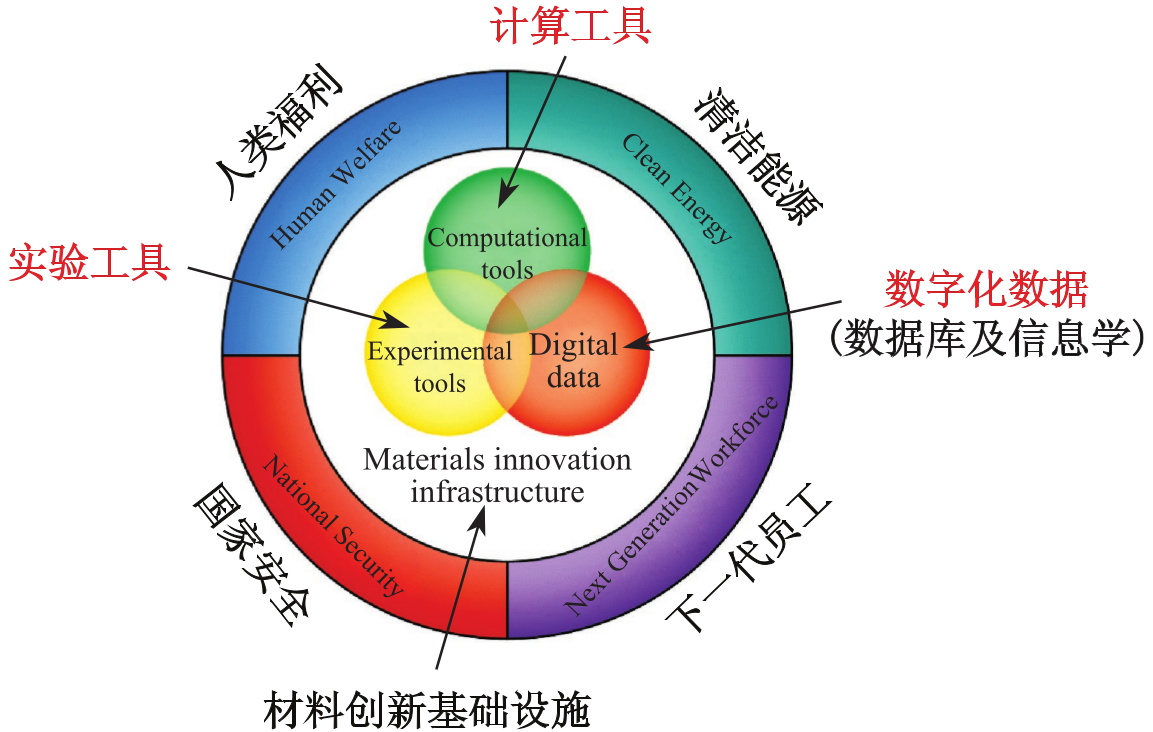
\includegraphics[height=2.55in,width=4.05in]{Figures/MGE.png}
%\caption{\tiny \textrm{Pseudopotential for metallic sodium, based on the empty core model and screened by the Thomas-Fermi dielectric function.}}%(与文献\cite{EPJB33-47_2003}图1对比)
%\caption{\tiny \textrm{Pseudopotential for metallic sodium, based on the empty core model and screened by the Thomas-Fermi dielectric function.}}%(与文献\cite{EPJB33-47_2003}图1对比)
\label{MGE}
\end{figure}
}

\frame
{
	\frametitle{材料模拟的基本思想和方法}
\begin{figure}[h!]
\vspace*{-0.25in}
\centering
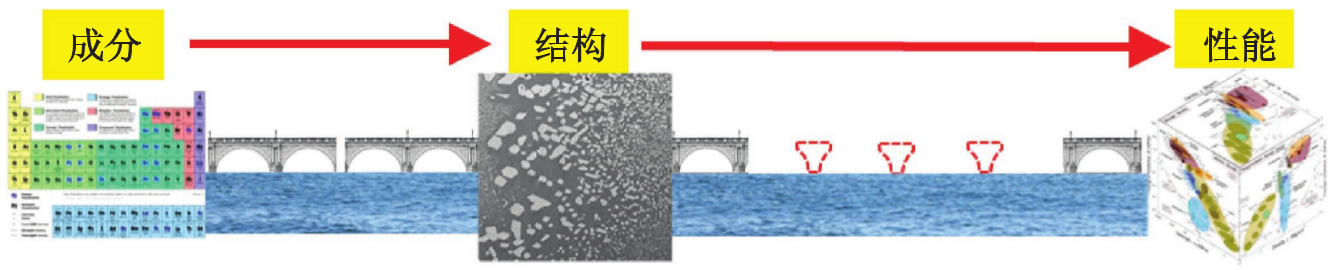
\includegraphics[height=0.80in,width=4.05in]{Figures/MGE-2.png}
%\caption{\tiny \textrm{Pseudopotential for metallic sodium, based on the empty core model and screened by the Thomas-Fermi dielectric function.}}%(与文献\cite{EPJB33-47_2003}图1对比)
\vskip 0.05pt
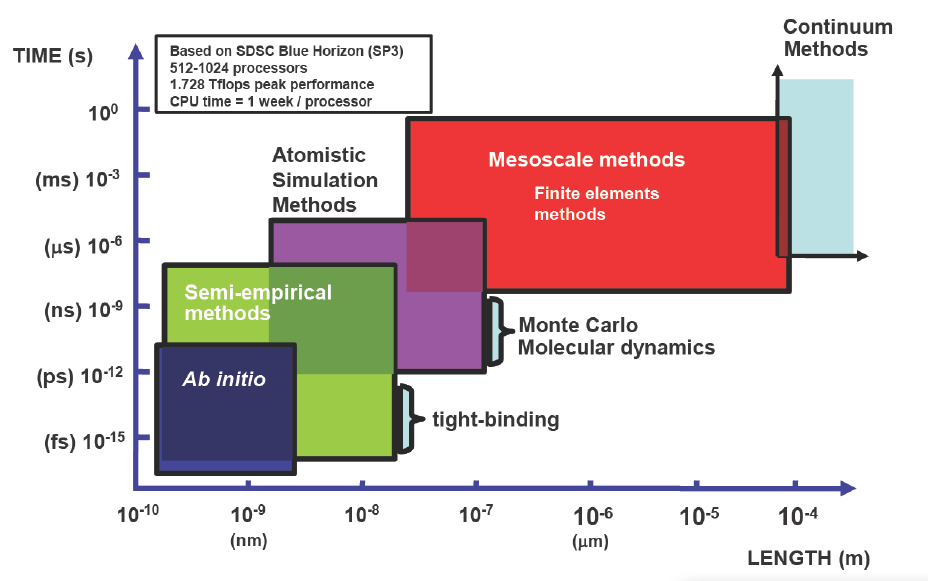
\includegraphics[height=2.20in,width=3.45in]{Figures/Multi-Scale-6.png}
%\caption{\tiny \textrm{Pseudopotential for metallic sodium, based on the empty core model and screened by the Thomas-Fermi dielectric function.}}%(与文献\cite{EPJB33-47_2003}图1对比)
\label{Multi-Scale}
\end{figure}
}

\frame
{
	\frametitle{\rm{I~Have~A~Dream}}
\begin{figure}[h!]
\vspace*{-0.18in}
\centering
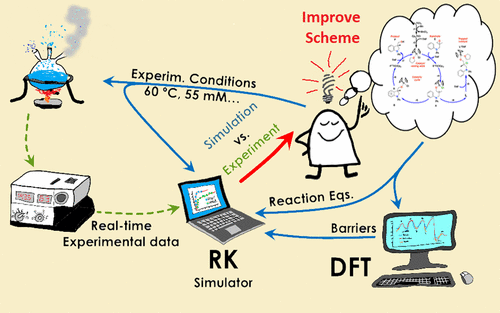
\includegraphics[height=2.55in,width=4.05in]{Figures/Schematic_Material-Design.png}
%\caption{\tiny \textrm{Pseudopotential for metallic sodium, based on the empty core model and screened by the Thomas-Fermi dielectric function.}}%(与文献\cite{EPJB33-47_2003}图1对比)
%\caption{\tiny \textrm{Pseudopotential for metallic sodium, based on the empty core model and screened by the Thomas-Fermi dielectric function.}}%(与文献\cite{EPJB33-47_2003}图1对比)
\label{Schematic_Material-Design}
\end{figure}
}

\frame
{
	\frametitle{\textit{ab~initio}和\textrm{first~principle}}
	\begin{itemize}
		\item \textit{ab~initio}是拉丁文词汇\textrm{(Latin~term)},其含义是\textrm{``from the beginning''},由拉丁文\textit{ab}~\textrm{(``from'')}+\textit{initio}~\textrm{(``beginning'')}合成,后者是\textit{initium}的单数夺格\footnote{\fontsize{5.5pt}{4.2pt}\selectfont{夺格\textrm{(ablative)},又称离格或从格,语法功能上表示某些词汇的状语。拉丁文\textit{initium}的意思是''开始、初始''。}}
		\item \textit{ab~initio}常用于法律和科学领域,如从头计算法(\textit{ab~initio}~\textrm{method})。法律中,\textit{ab~initio}表示"一开始即如此,而非法院宣判之后"。
		\item \textrm{first~principle}指从基本的物理学定律出发,不外加假设与经验拟合的推导与计算。
		\item 在物理学领域,\textrm{first~principle}(第一性原理)和\textit{ab~initio}(从头计算)含义上是等价的。例如利用\textrm{Schr\"odinger}方程在一些近似条件下求解电子结构,但无须依赖实验数据得到拟合参数的方法,就是第一原理或从头计算法。
	\end{itemize}
}

\frame
{
	\frametitle{\textit{ab~initio} \textrm{in inscription}}
\begin{figure}[h!]
\vspace*{-0.15in}
\centering
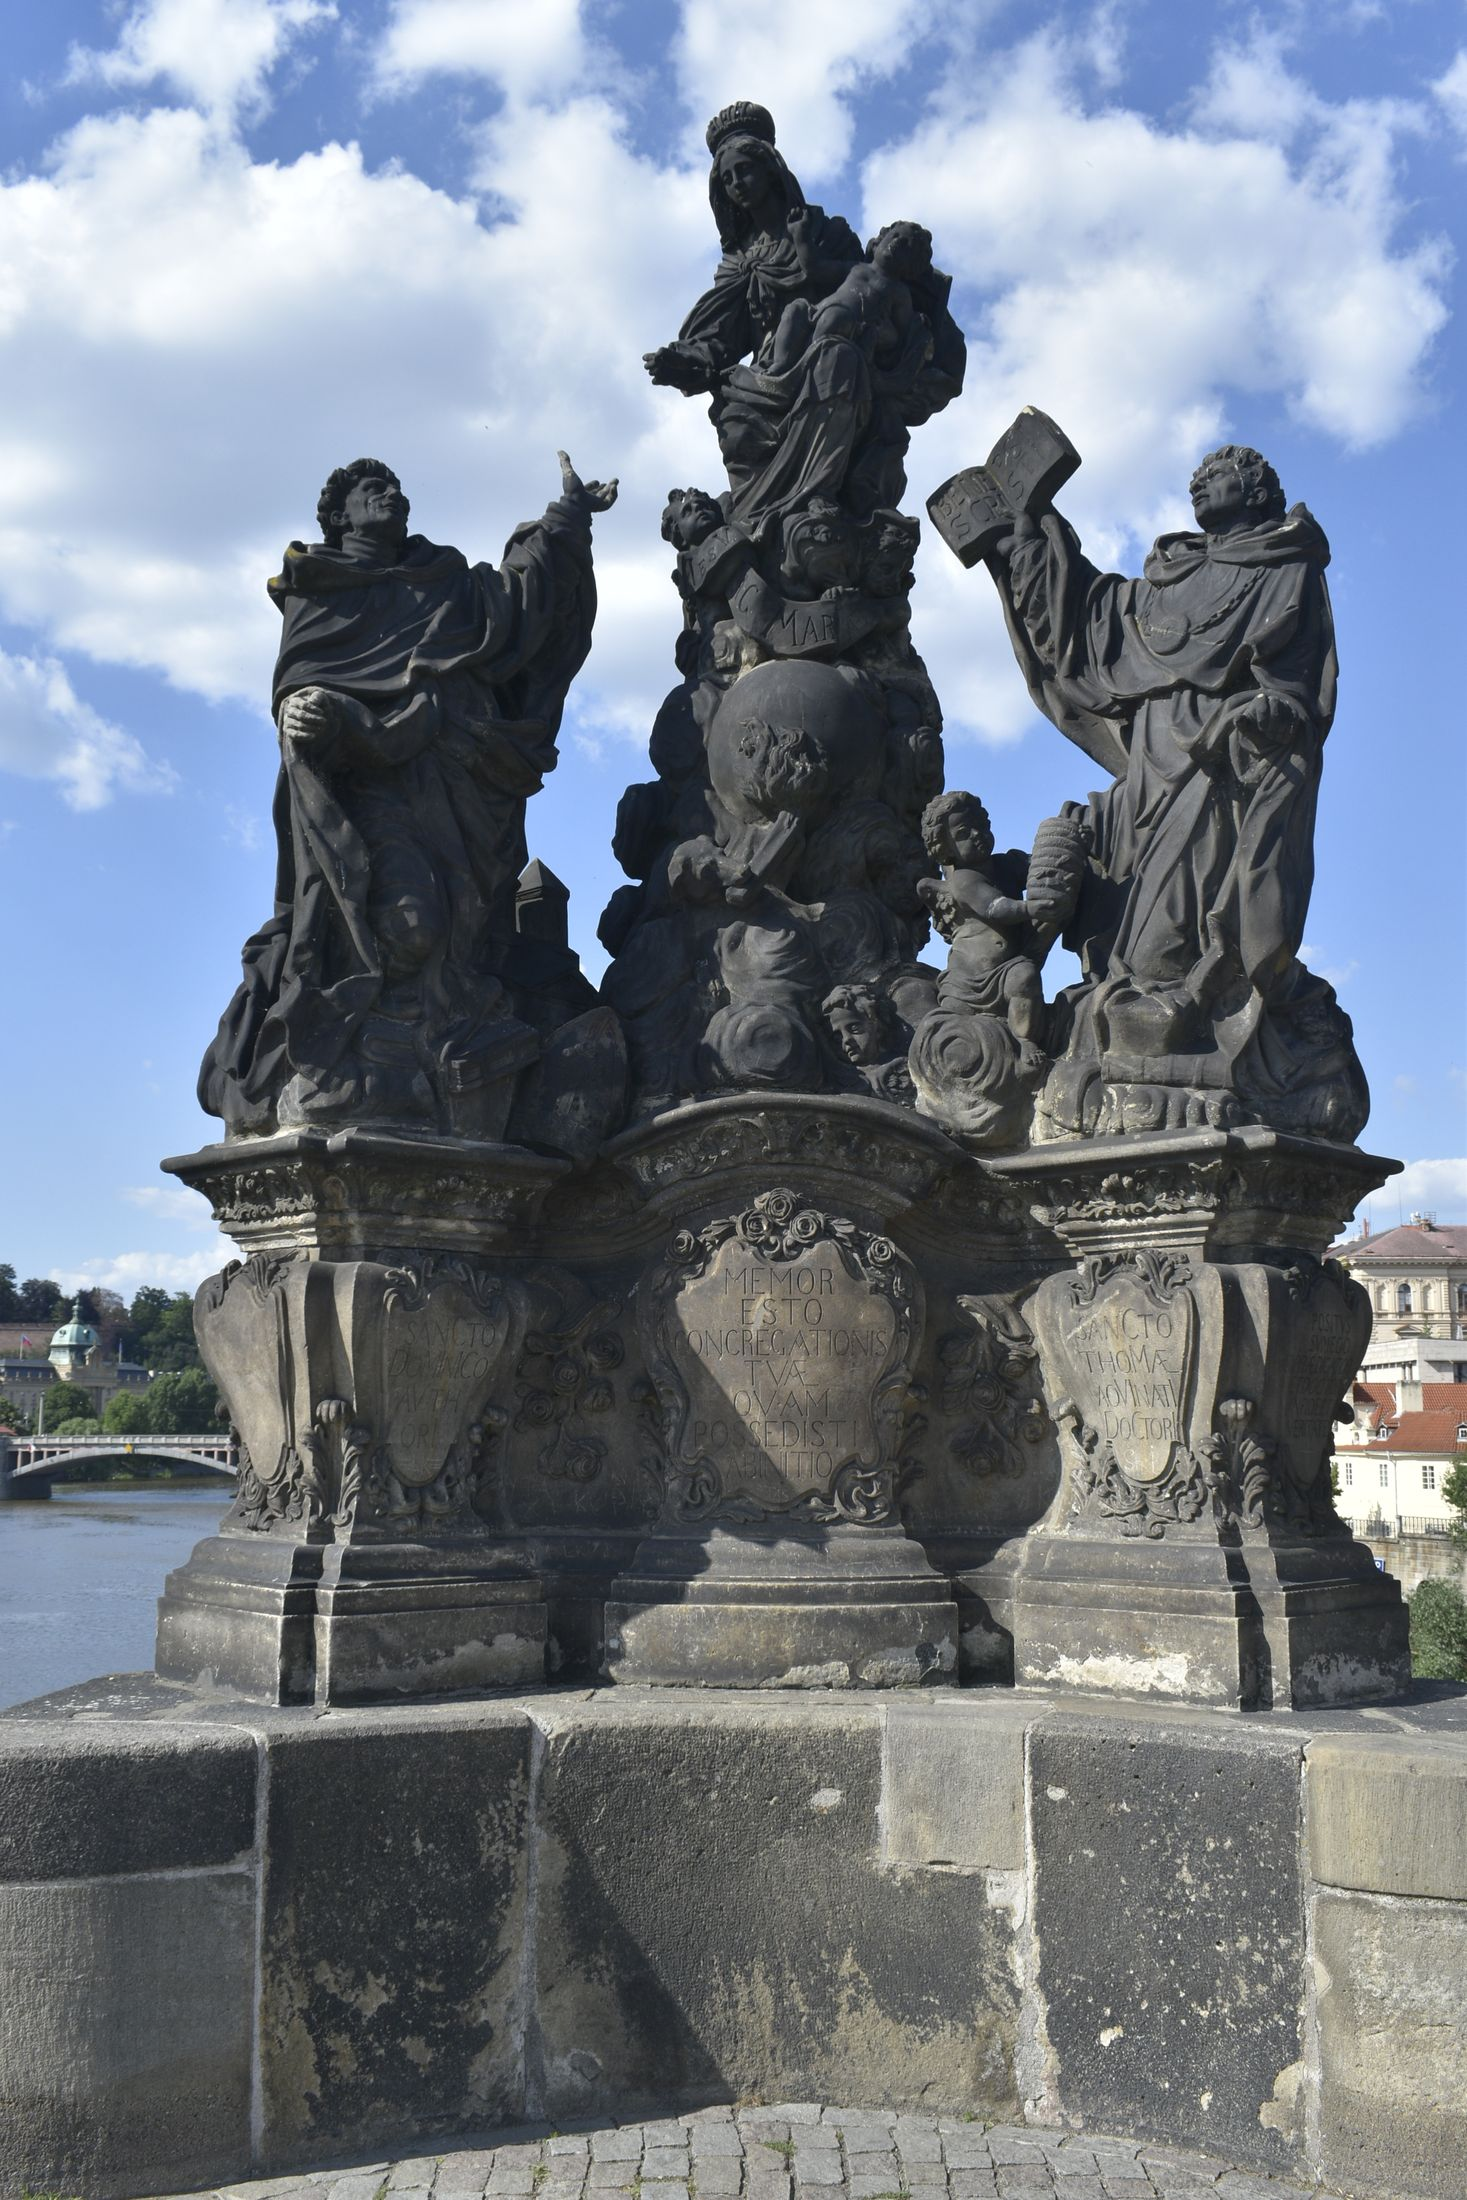
\includegraphics[height=2.10in,width=1.55in,viewport=5 3 1550 2180,clip]{Figures/Madonna-Ss.-Dominic-and-Thomas_Aquinas-3.jpeg}
\hspace*{15pt}
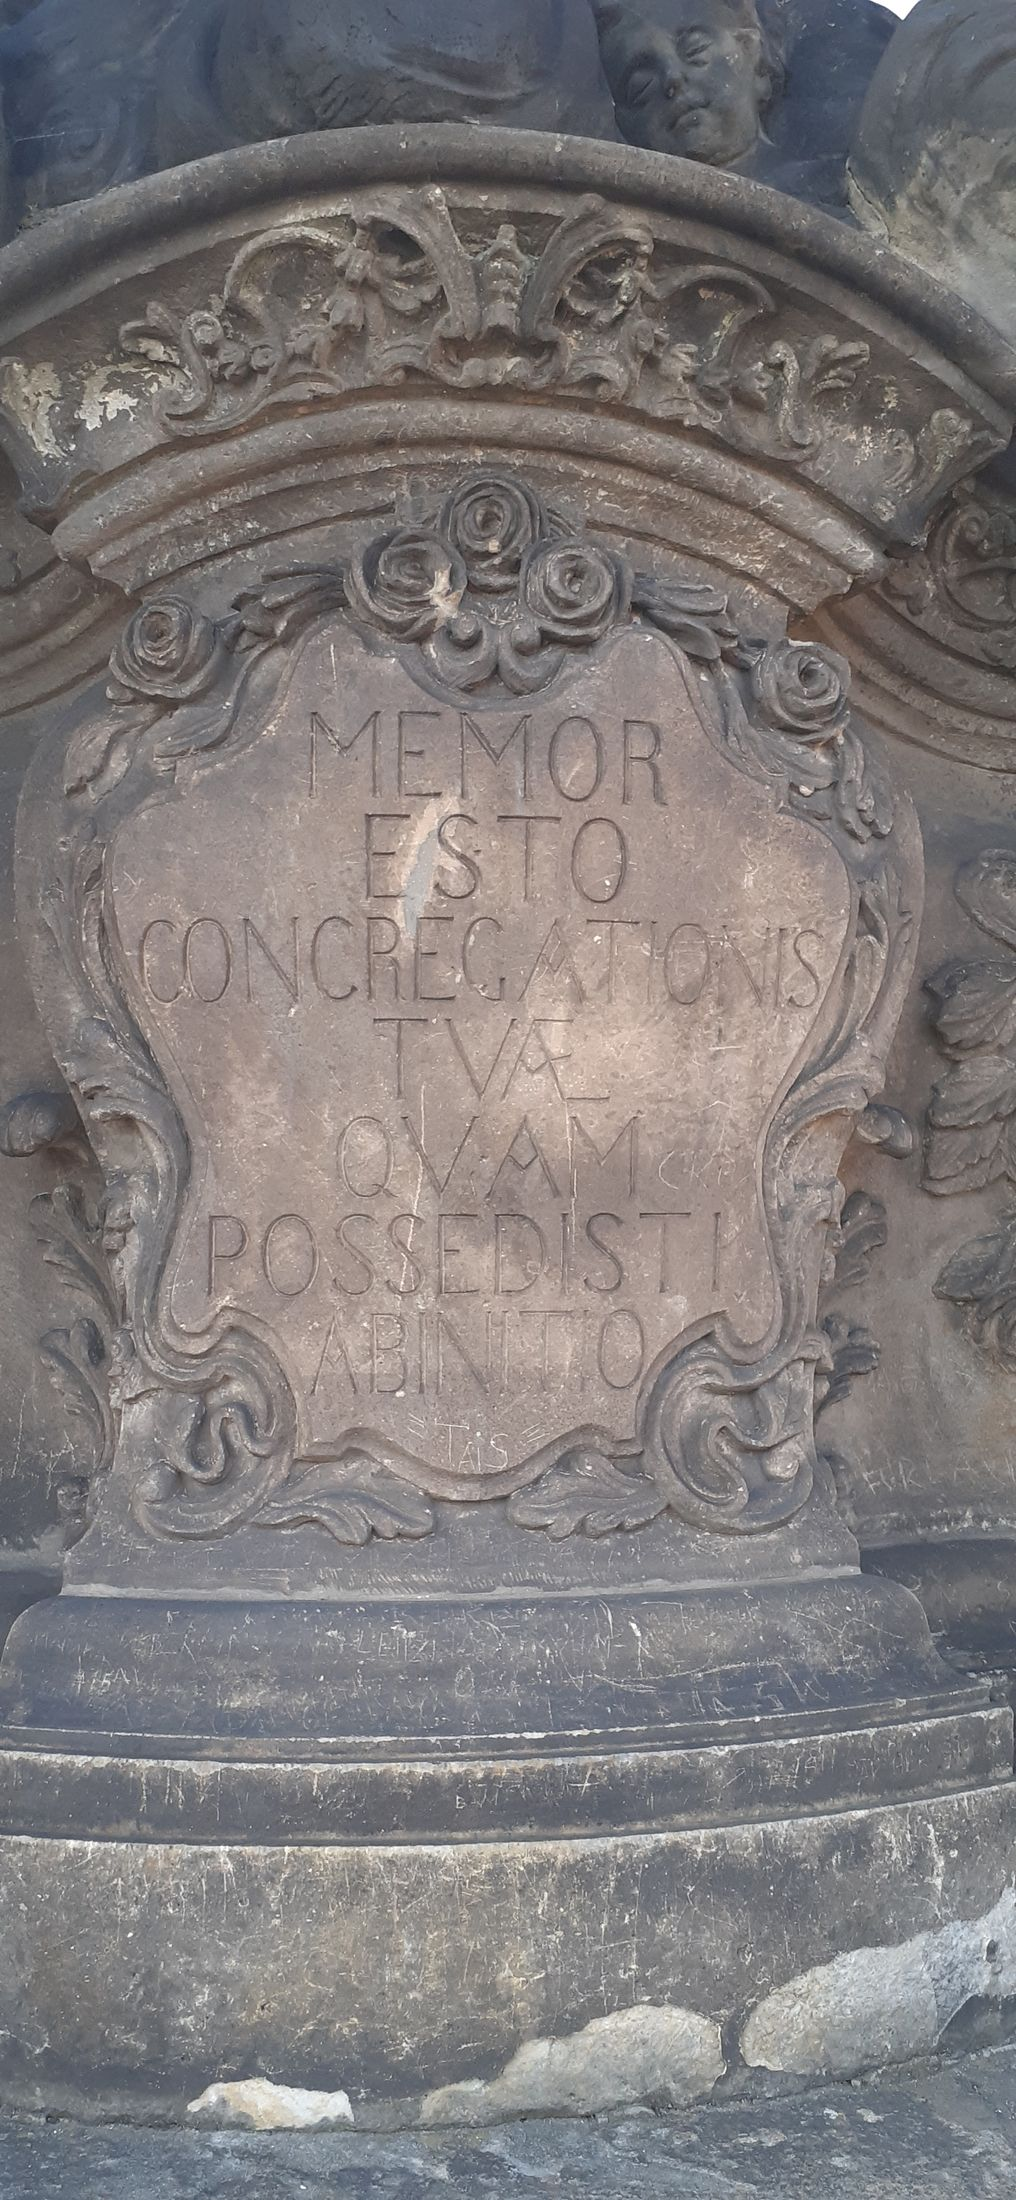
\includegraphics[height=2.10in,width=1.15in,viewport=5 3 950 1880,clip]{Figures/Madonna-Ss.-Dominic-and-Thomas_Aquinas-Inscription_2.jpeg}
%\caption{\tiny \textrm{Pseudopotential for metallic sodium, based on the empty core model and screened by the Thomas-Fermi dielectric function.}}%(与文献\cite{EPJB33-47_2003}图1对比)
\label{ABINITIO-inscription}
\end{figure}
\begin{minipage}{0.53\textwidth}
	{\fontsize{8.2pt}{4.2pt}\selectfont{ 
		\centering{MEMOR}\\
		\centering{ESTO}\\
		\centering{CONGREGATIONIS}\\
		\centering{TV\AE}\\
		\centering{QVAM}\\
		\centering{POSSEDISTI}\\
		\centering{\textcolor{red}{ABINITO}\\}}}
\end{minipage}
\hspace*{5pt}
\begin{minipage}{0.30\textwidth}
	\textrm{\fontsize{4.2pt}{4.2pt}\selectfont{The inscription in English:}}\\
	\textrm{\fontsize{8.2pt}{4.2pt}\selectfont{\textcolor{blue}{Mind the congregation that has been yours} \textcolor{purple}{since the beginning}}}
\end{minipage}
}

%-----------------------------------------------------------------------------------------------------------------------------------------------------------------------%
\section{量子力学基础}
\subsection{能量量子化}
\frame
{
	\frametitle{经典物理学的成功}
\begin{figure}[h!]
\vspace*{-0.18in}
\centering
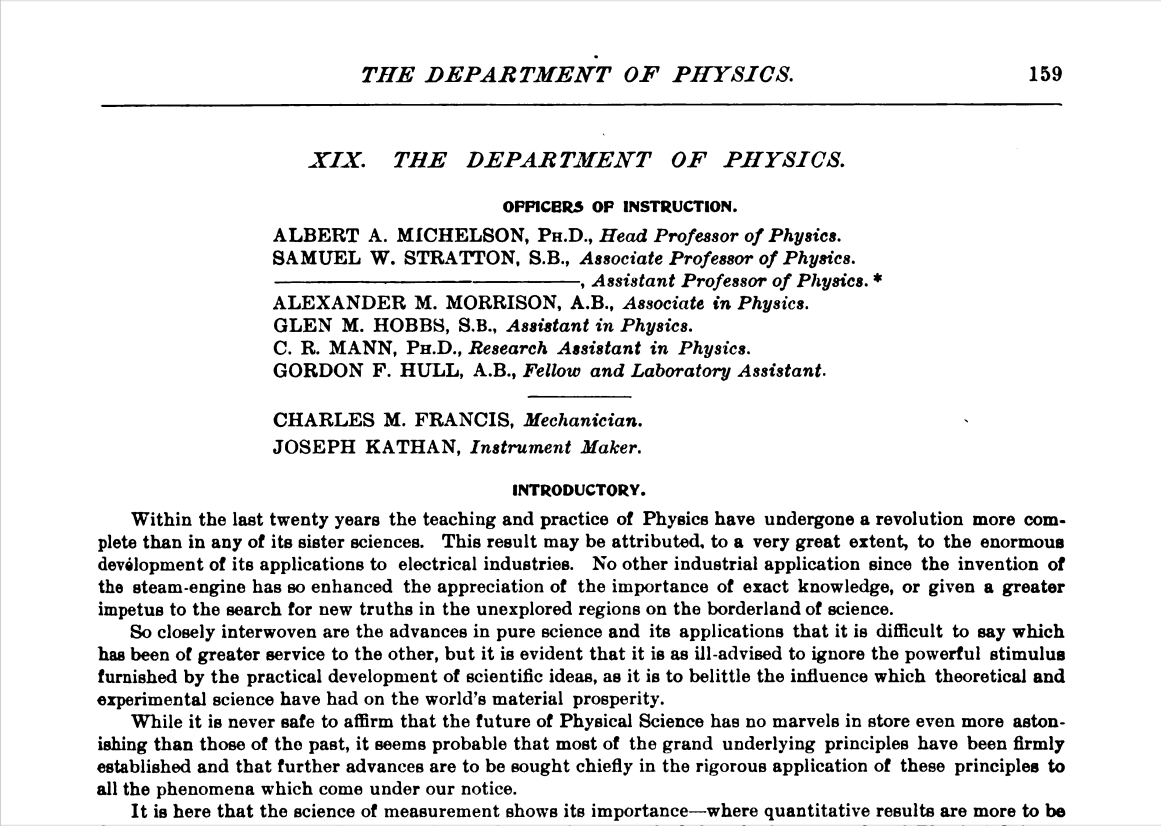
\includegraphics[height=1.90in,width=3.00in,viewport=0 0 1150 690,clip]{Figures/Albert_Michelson-Quotes.jpg}
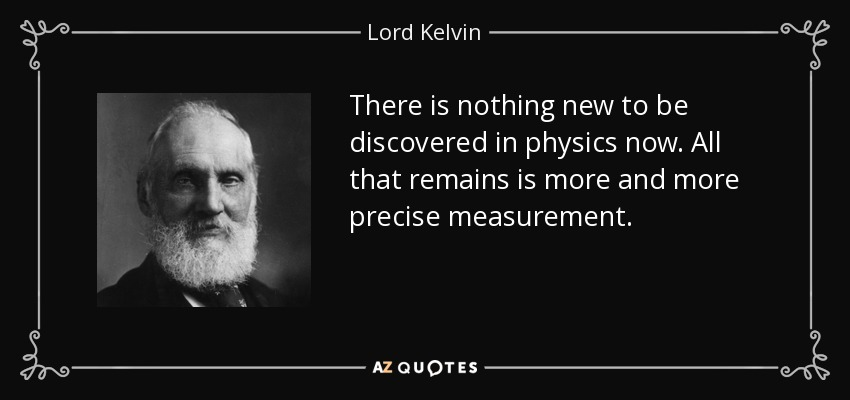
\includegraphics[height=1.10in,width=2.55in,viewport=0 0 880 400,clip]{Figures/Quote-there-is-nothing-new-to-be-discovered-in-physics-now-all-that-remains-is-more-and-more-lord-kelvin-57-38-79.jpg}
%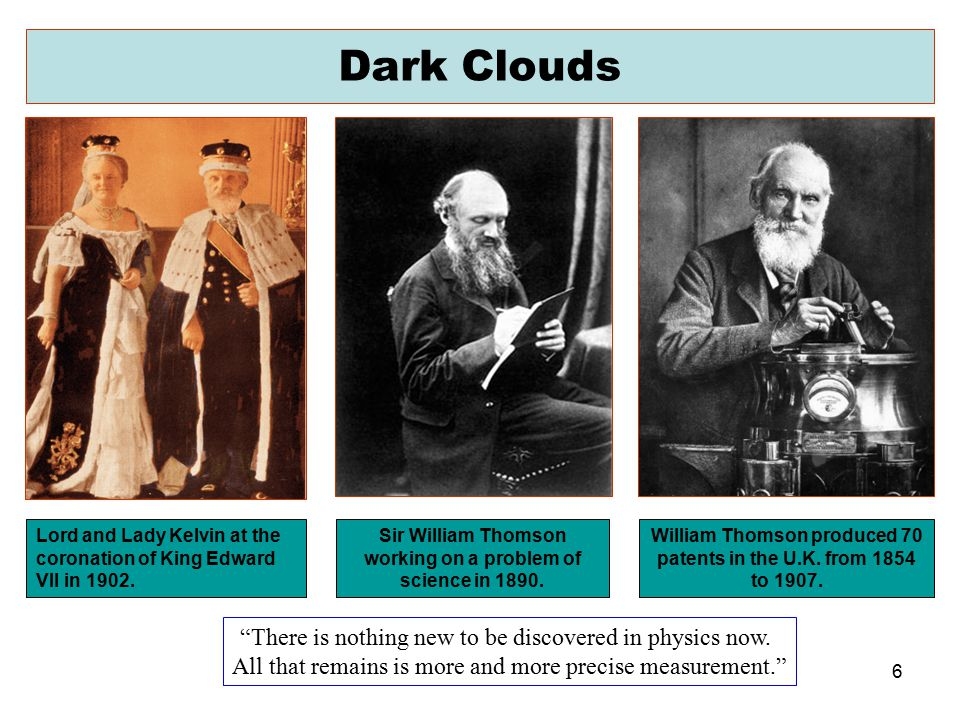
\includegraphics[height=2.50in,width=4.05in,viewport=0 20 735 470,clip]{Figures/Two-dark-cloud-in-physics-3.jpg}
%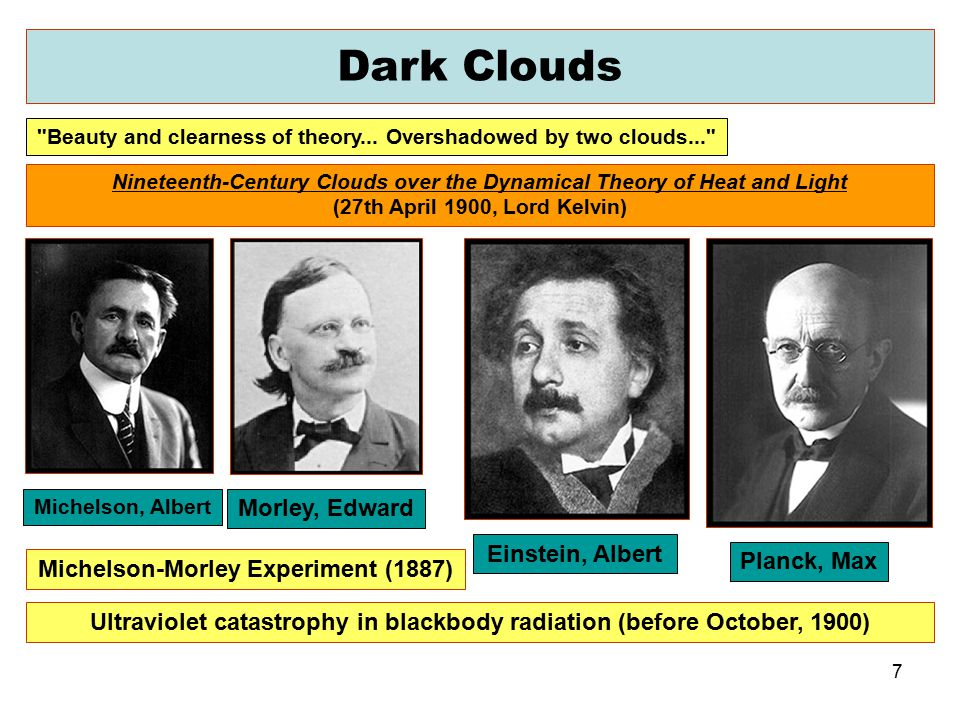
\includegraphics[height=2.40in,width=4.05in,viewport=0 50 735 470,clip]{Figures/Two-dark-cloud-in-physics-2.jpg}
%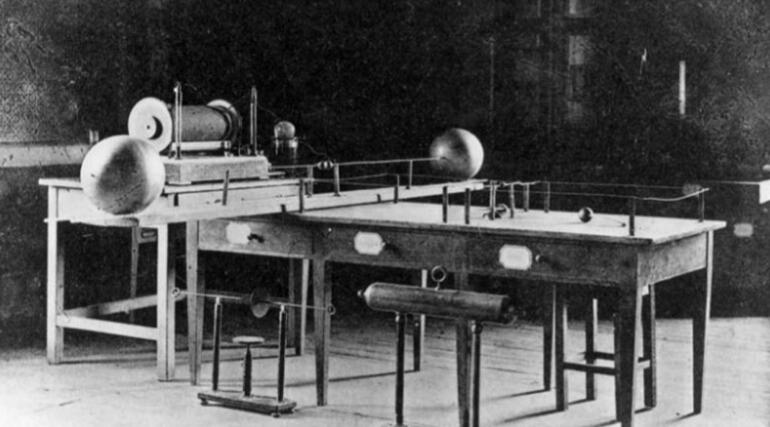
\includegraphics[height=2.40in,width=4.05in,viewport=0 0 580 325,clip]{Figures/Two-dark-cloud-in-physics-1.jpg}
\label{two_Dark_Clouds}
\end{figure}
}

\frame
{
	\frametitle{经典物理学天空的“两朵乌云”\textrm{(Dark Clouds)}}
\begin{figure}[h!]
\vspace*{-0.18in}
\centering
%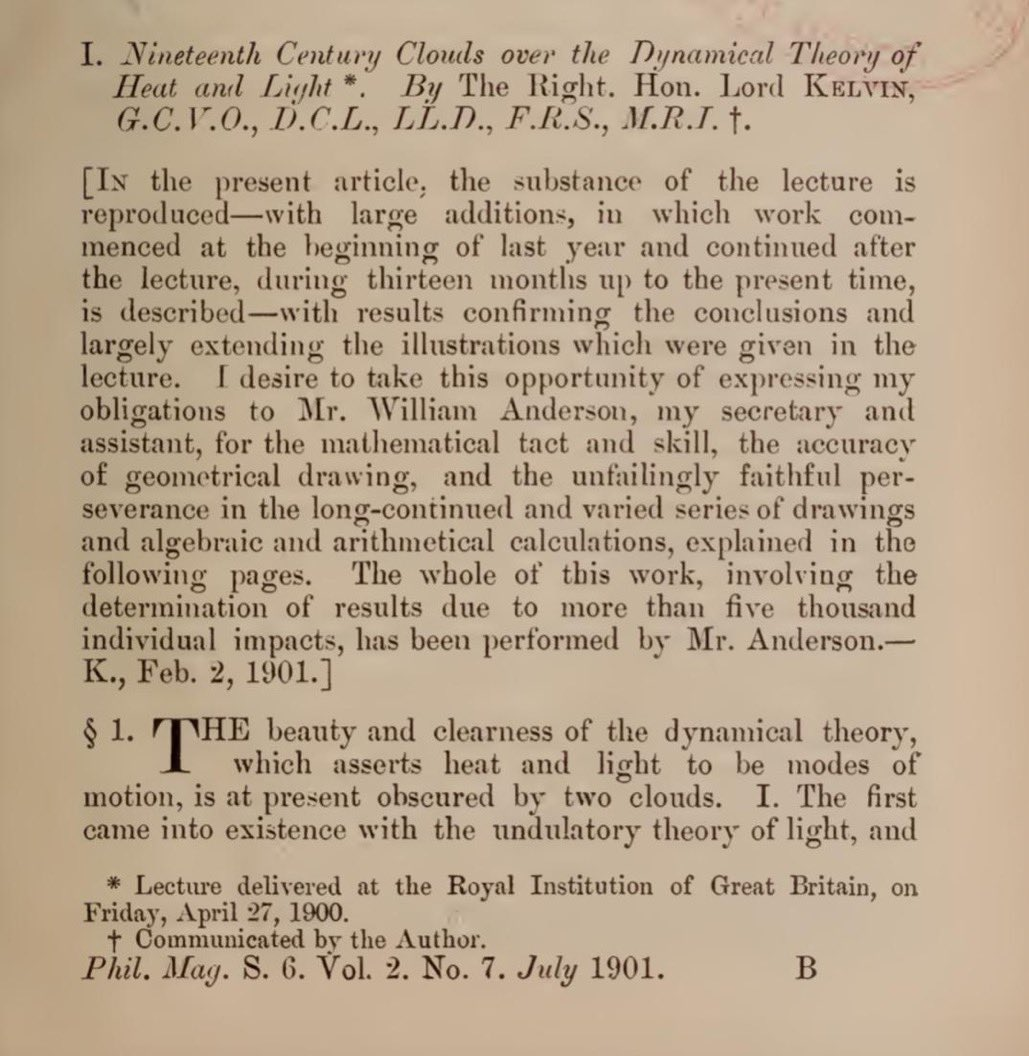
\includegraphics[height=2.90in,width=2.80in,viewport=0 0 1000 1100,clip]{Figures/Baron_Kelvin-Lecture.jpeg}
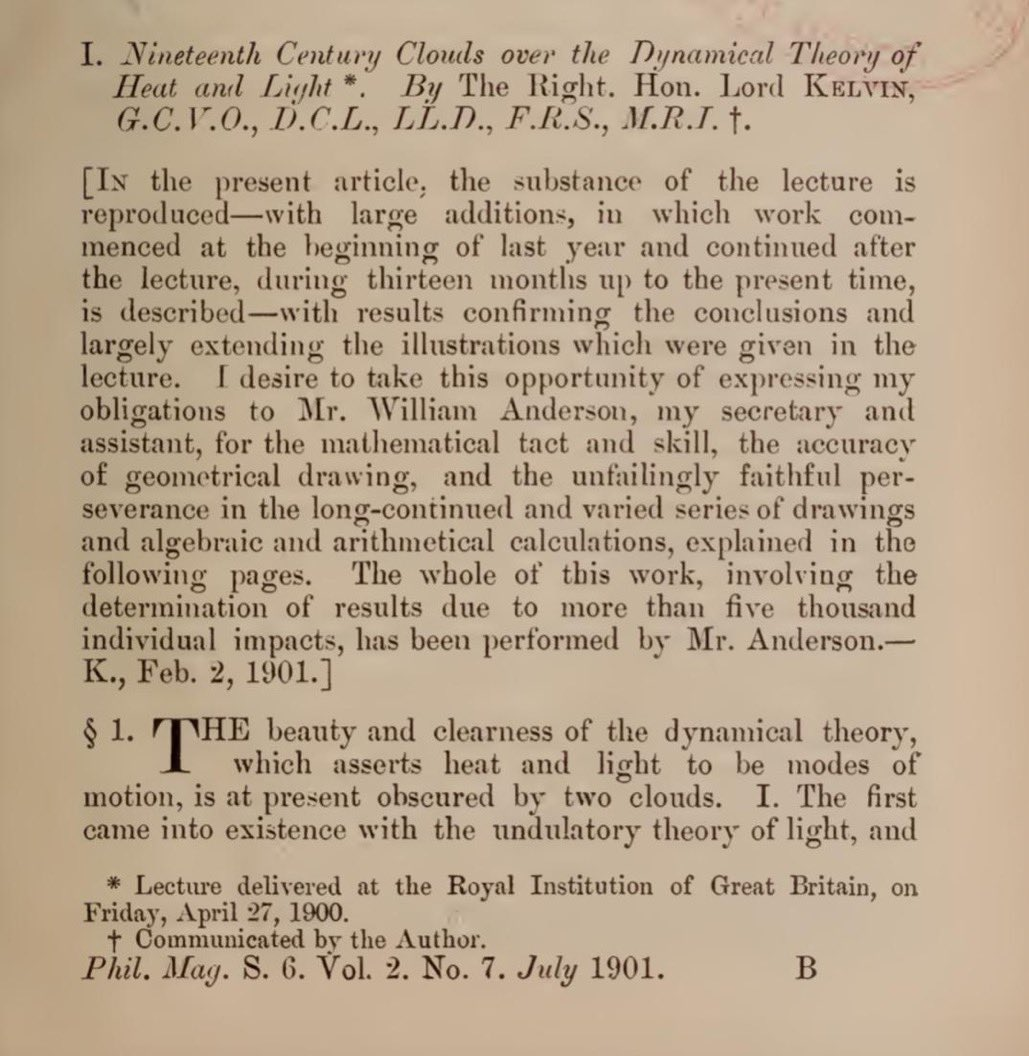
\includegraphics[height=0.35in,width=3.35in,viewport=0 900 1020 1030,clip]{Figures/Baron_Kelvin-Lecture.jpeg}
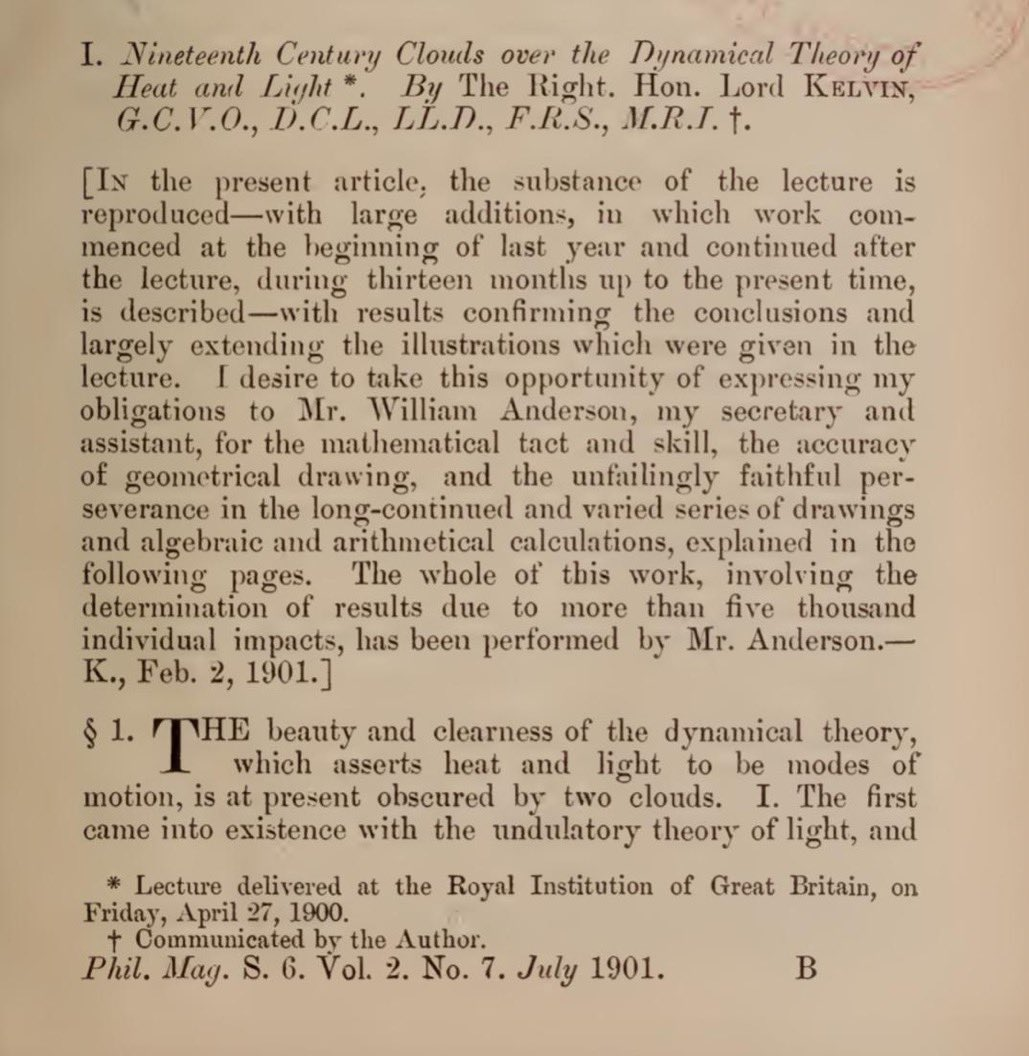
\includegraphics[height=0.80in,width=3.35in,viewport=0 50 1020 350,clip]{Figures/Baron_Kelvin-Lecture.jpeg}
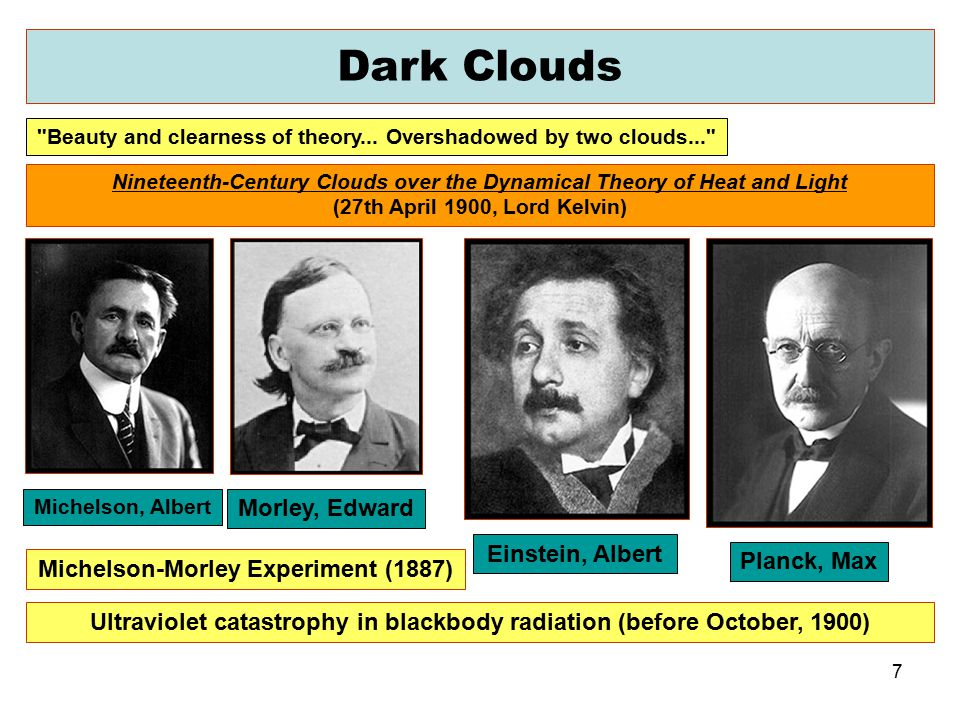
\includegraphics[height=1.85in,width=4.05in,viewport=0 50 735 370,clip]{Figures/Two-dark-cloud-in-physics-2.jpg}
\label{two_Dark_Clouds_2}
\end{figure}
}

%\frame
%{
%	\frametitle{经典物理学天空的“两朵乌云”\textrm{(Dark Clouds)}}
%\begin{figure}[h!]
%\vspace*{-0.18in}
%\centering
%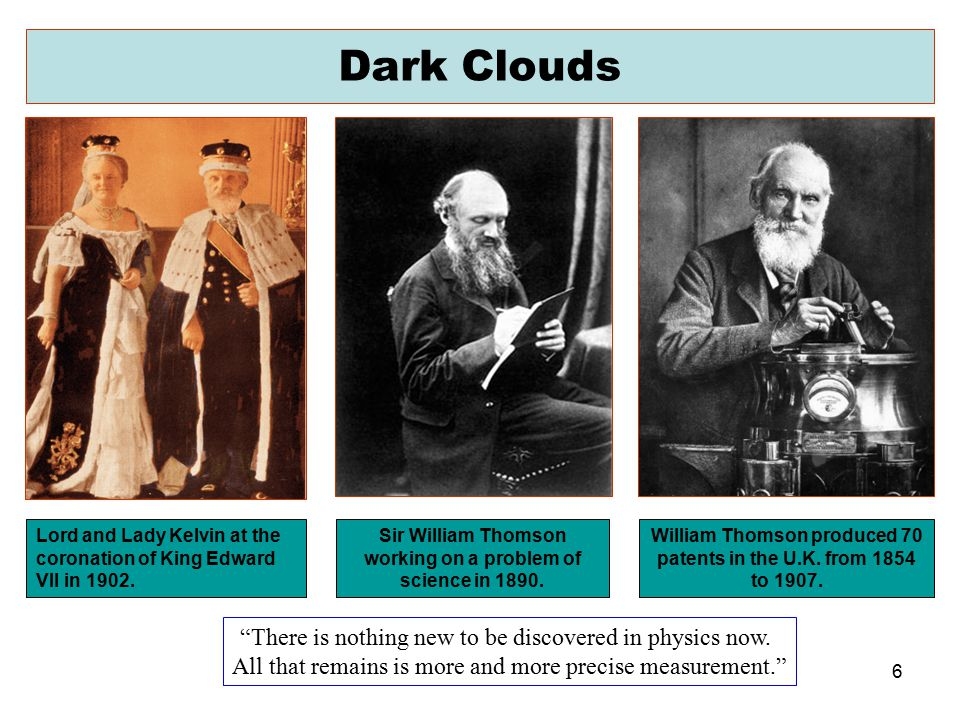
\includegraphics[height=2.50in,width=4.05in,viewport=0 20 735 470,clip]{Figures/Two-dark-cloud-in-physics-3.jpg}
%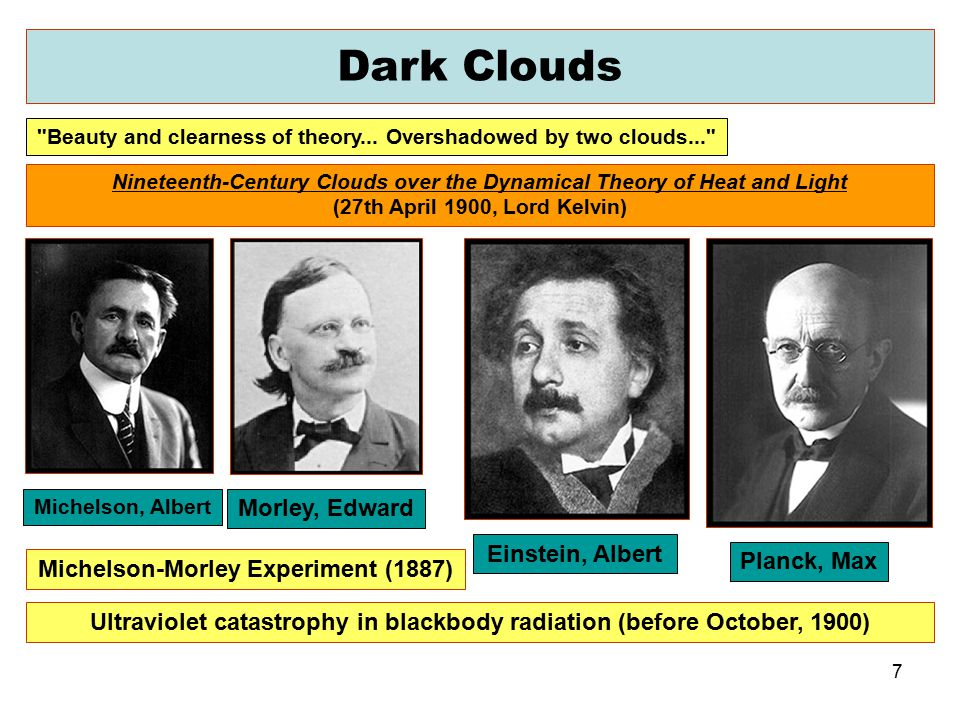
\includegraphics[height=2.40in,width=4.05in,viewport=0 50 735 470,clip]{Figures/Two-dark-cloud-in-physics-2.jpg}
%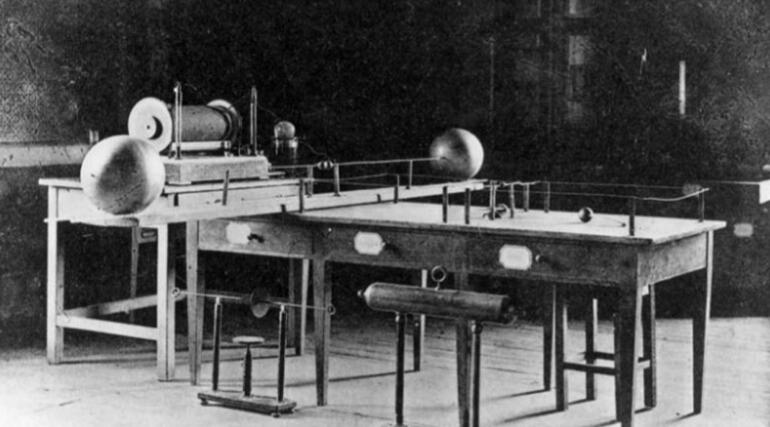
\includegraphics[height=2.40in,width=4.05in,viewport=0 0 580 325,clip]{Figures/Two-dark-cloud-in-physics-1.jpg}
%\label{two_Dark_Clouds_3}
%\end{figure}
%}
%
\frame
{
	\frametitle{黑体辐射与能量量子化}
	\textrm{1900}年,为了解释黑体辐射\textrm{(black-body radiation)}的能量密度与电磁辐射频率的关系,\textrm{M.~Planck}%放弃\textcolor{blue}{能量均分定理}\textrm{(the equipartition theorem)},
	引入\textcolor{red}{能量量子化}\textrm{(quantization of energy)}的假设,利用统计物理推导出与实验符合得非常好的黑体辐射\textrm{Planck~}公式:~
	\begin{displaymath}
		\rho_{\nu}\mathrm{d}{\nu}=\dfrac{8{\pi}h{\nu}^3}{C^2}\bigg(\dfrac1{\mathrm{e}^{h\nu/kT}-1}\bigg)\mathrm{d}\nu
	\end{displaymath}
\begin{figure}[h!]
\centering
\vspace{-10.5pt}
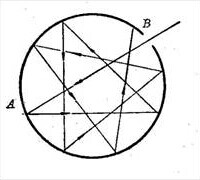
\includegraphics[height=1.45in,width=1.45in,viewport=0 0 136 136,clip]{Figures/Black_box.jpg}
\hskip 1pt
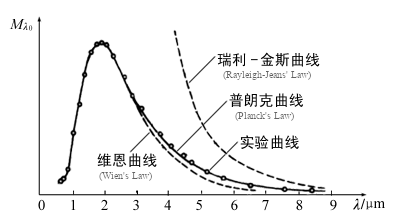
\includegraphics[height=1.32in,width=2.25in,viewport=0 0 390 215,clip]{Figures/Black_box_curve.png}
\caption{\textrm{The black-body radiation and the curve}}
\label{Black_box}
\end{figure}
}

\frame
{
	\frametitle{波-粒二象性与光电效应}
\begin{figure}[h!]
\centering
\vspace{-15.5pt}
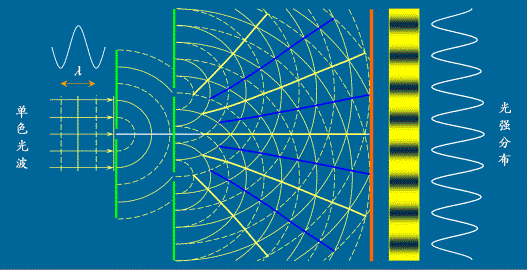
\includegraphics[height=1.35in,width=2.70in,viewport=0 0 536 280,clip]{Figures/wave-particle_duality.png}
\vskip 1pt
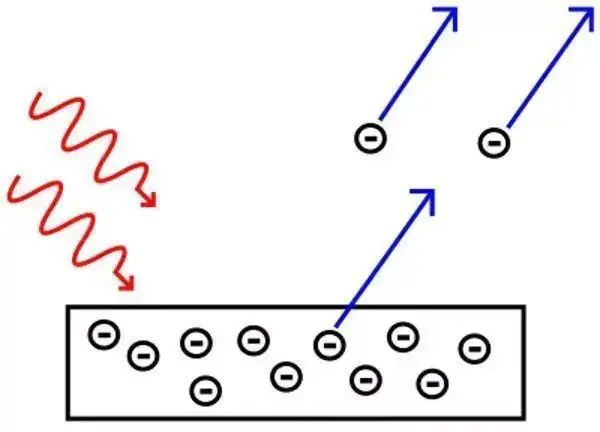
\includegraphics[height=1.32in,width=2.05in,viewport=0 0 620 455,clip]{Figures/Photoelectic_effect.png}
\caption{\textrm{The wave-particle duality and Photoelectric effect}}
\label{wave_and_particle}
\end{figure}
}

\frame
{
	\frametitle{电子衍射、\textrm{Compton~effect}与\textrm{H}原子光谱}
\begin{figure}[h!]
\centering
\vspace{-15.5pt}
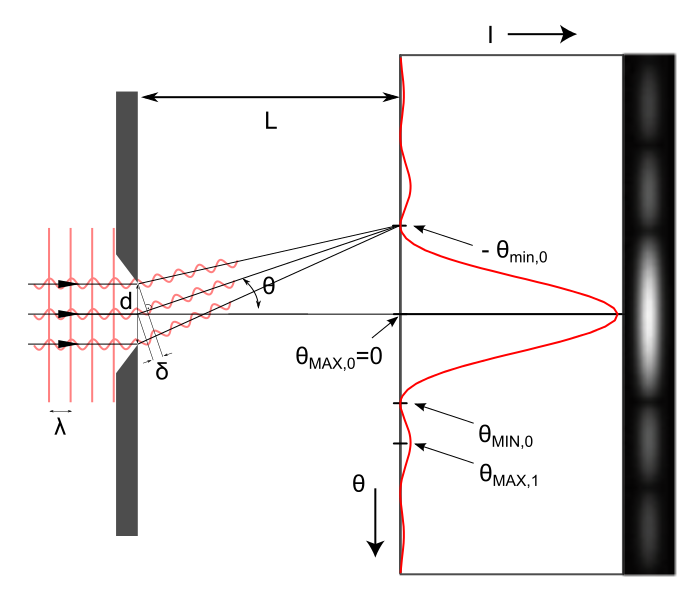
\includegraphics[height=1.35in,width=1.80in,viewport=0 0 680 600,clip]{Figures/Single_Slit_Diffraction.png}
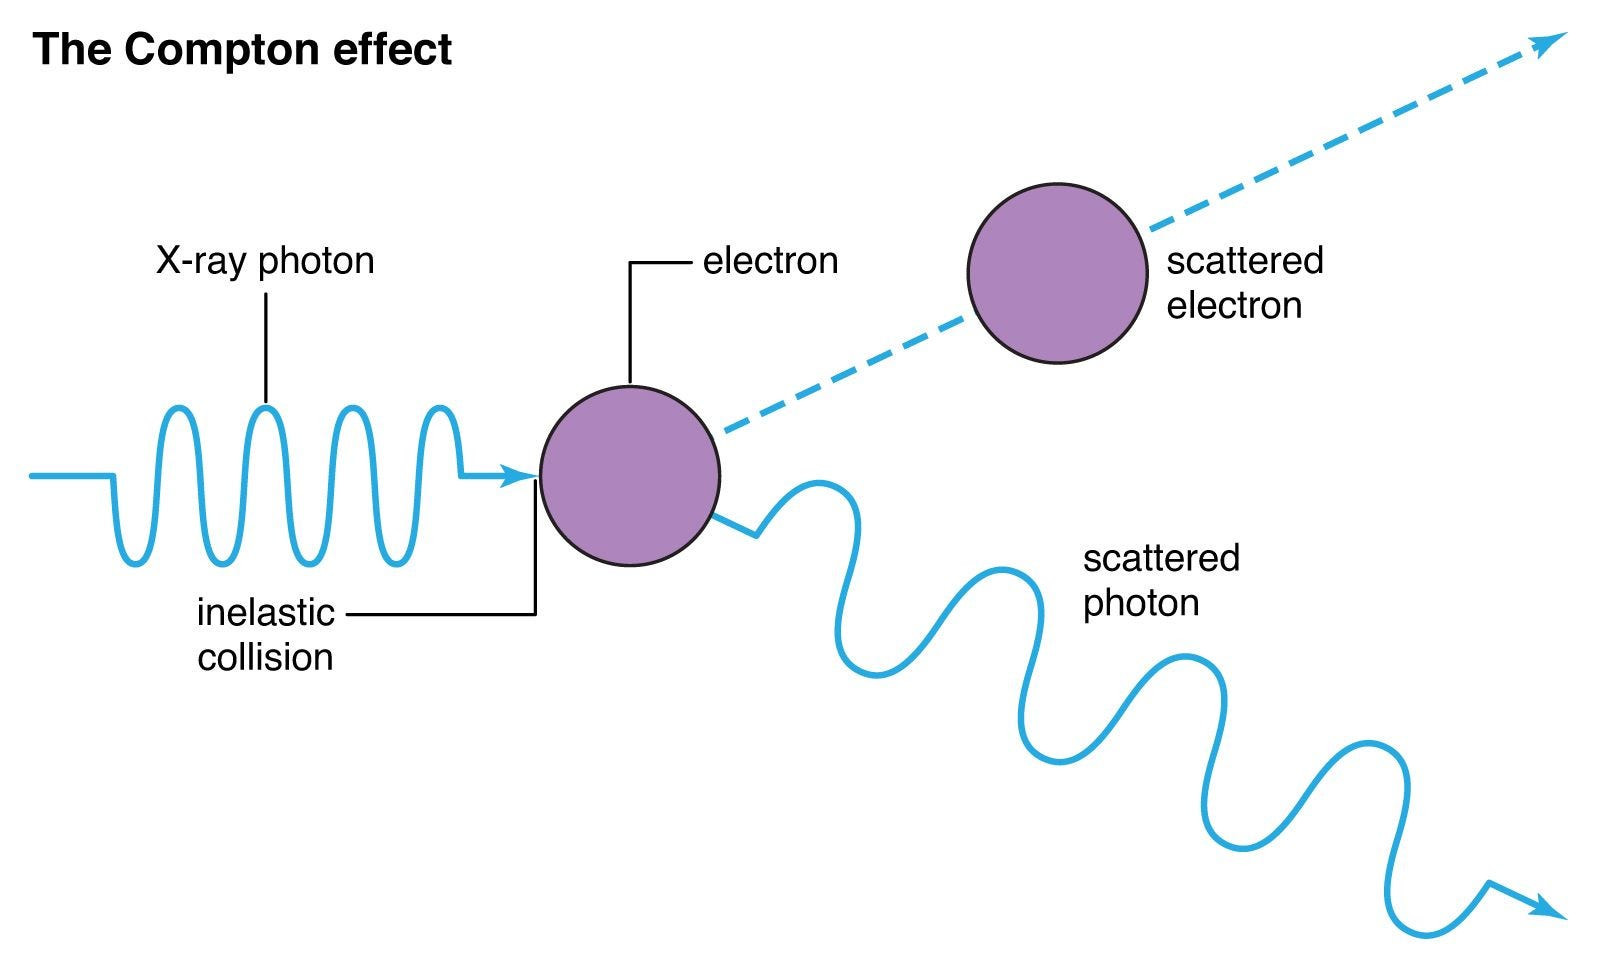
\includegraphics[height=1.20in,width=2.10in,viewport=0 0 1600 950,clip]{Figures/Compton_effect.jpg}\\
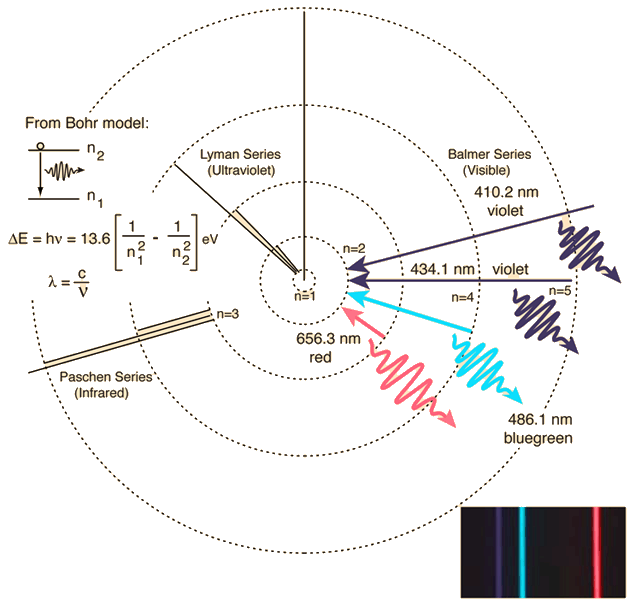
\includegraphics[height=1.65in,width=1.75in,viewport=0 0 620 600,clip]{Figures/Hydrogen_spectrum-3.png}
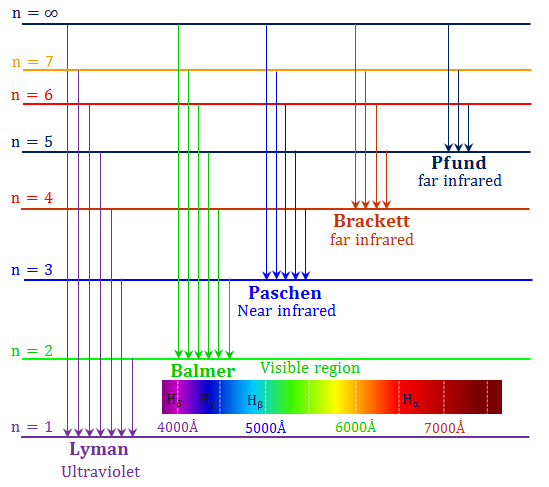
\includegraphics[height=1.55in,width=1.75in,viewport=0 0 500 380,clip]{Figures/Hydrogen_spectrum-2.png}
%\caption{\textrm{The wave-particle duality and Photoelectric effect}}
\label{electron:wave_and_particle}
\end{figure}
}

\subsection{\textrm{Schr\"odinger}方程与量子力学的建立}
\frame
{
	\frametitle{\textrm{De Broglie}物质波}
\begin{minipage}{0.53\textwidth}
\begin{figure}[h!]
\centering
\vspace{-15.5pt}
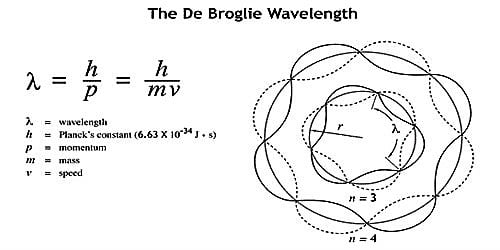
\includegraphics[height=1.3in,width=2.1in,viewport=0 0 500 280,clip]{Figures/De-Broglie-waves.jpg}
%\caption{\textrm{The wave-particle duality and Photoelectric effect}}
\label{Matter_wave}
\end{figure}
经典的观念:
\begin{itemize}
	\item \textcolor{red}{粒子}:~\textcolor{blue}{物质存在的形式}
	\item \textcolor{red}{波动}:~\textcolor{blue}{能量传递的形式}
\end{itemize}
\end{minipage}
\begin{minipage}{0.45\textwidth}
\begin{figure}[h!]
\centering
\vspace{-15.5pt}
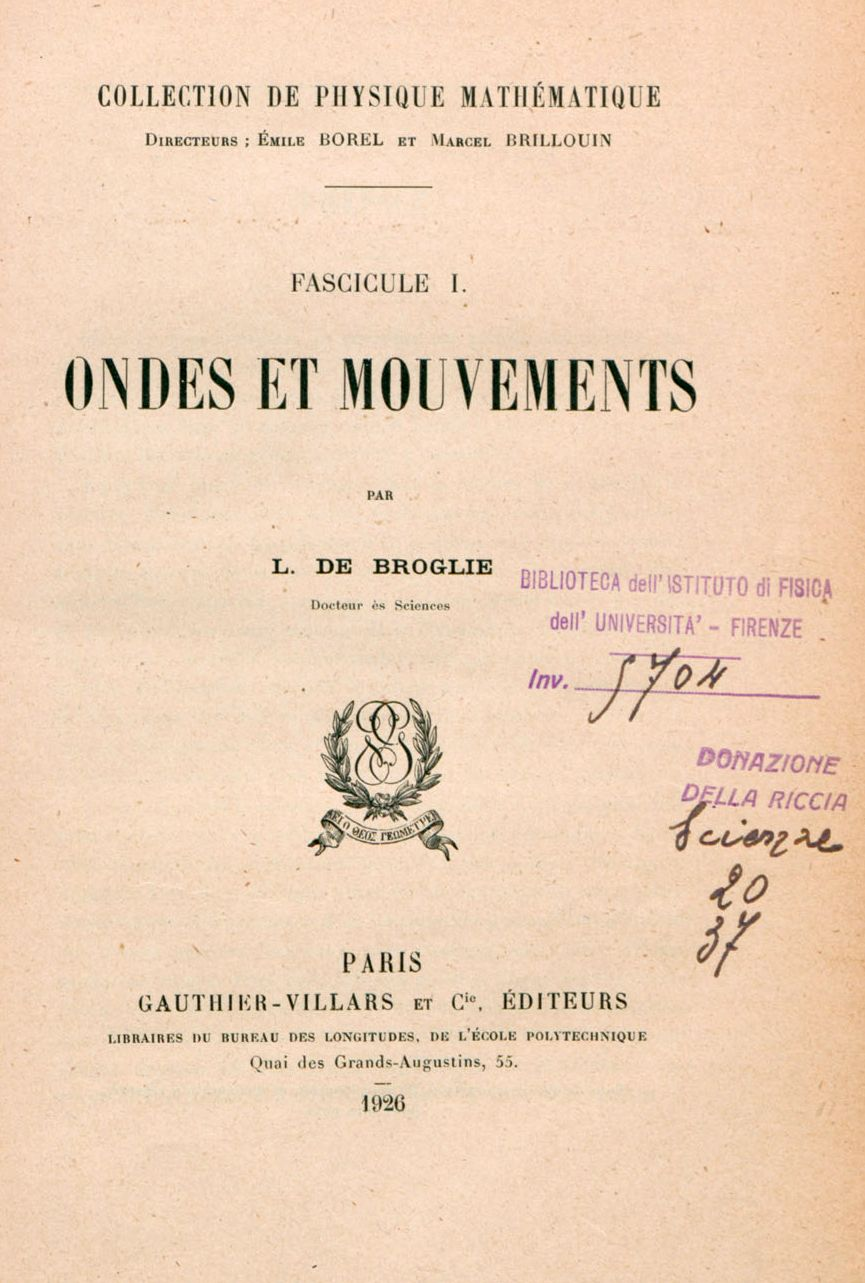
\includegraphics[height=2.80in,width=1.90in,viewport=0 0 430 650,clip]{Figures/De_Broglie-dissertation_Cover.jpg}
%\caption{\textrm{The wave-particle duality and Photoelectric effect}}
\label{De_Broglie-dissertation}
\end{figure}
\end{minipage}
}

\frame
{
	\frametitle{经典力学\textrm{Classical Mechanics}}
\begin{figure}[h!]
\vspace*{-0.18in}
\centering
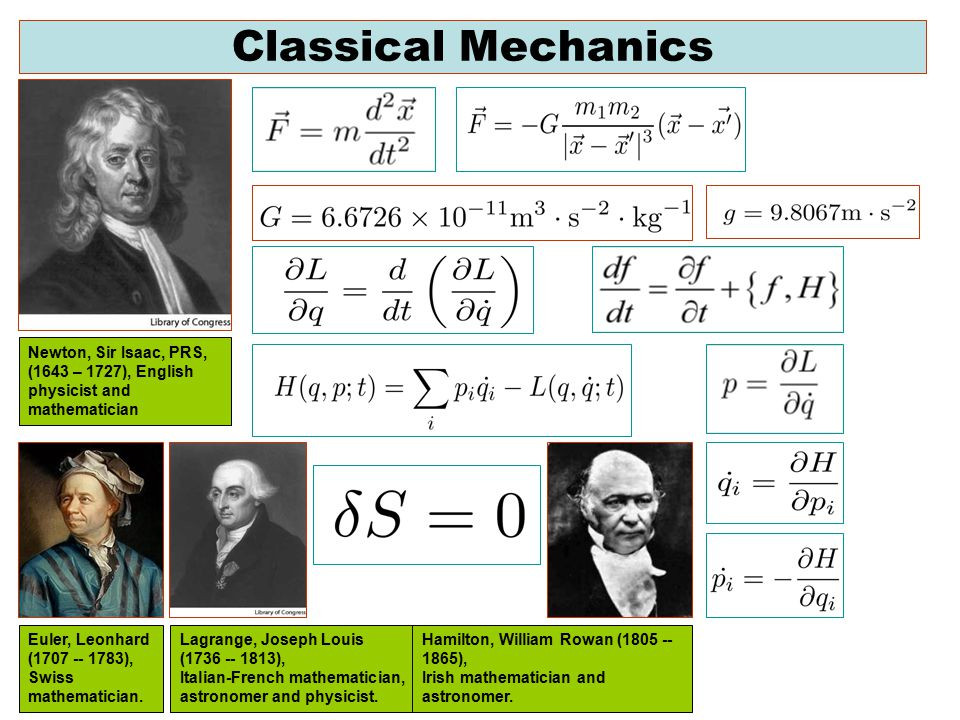
\includegraphics[height=2.65in,width=4.05in,viewport=0 0 715 495,clip]{Figures/Classical_Mechanics.jpg}
%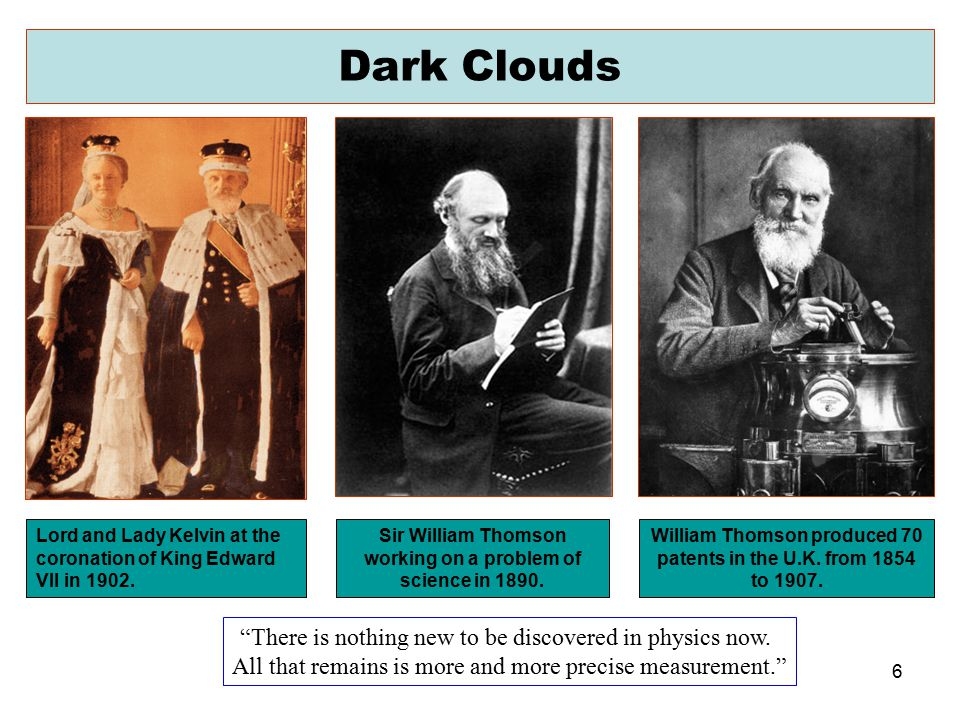
\includegraphics[height=2.50in,width=4.05in,viewport=0 20 735 470,clip]{Figures/Two-dark-cloud-in-physics-3.jpg}
%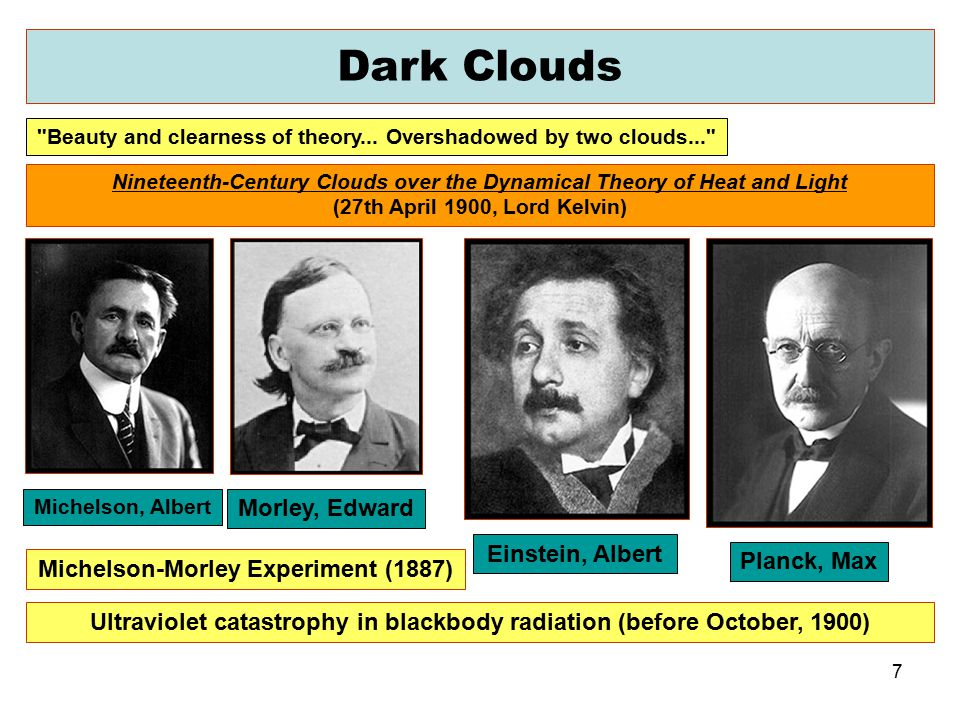
\includegraphics[height=2.40in,width=4.05in,viewport=0 50 735 470,clip]{Figures/Two-dark-cloud-in-physics-2.jpg}
%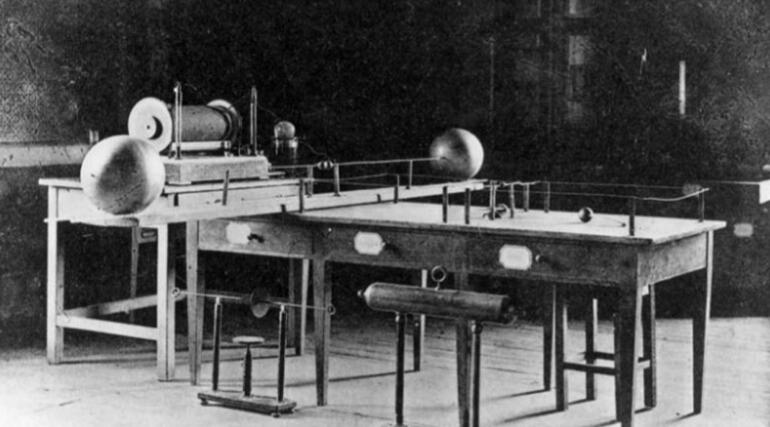
\includegraphics[height=2.40in,width=4.05in,viewport=0 0 580 325,clip]{Figures/Two-dark-cloud-in-physics-1.jpg}
\label{Classical_Mechanics}
\end{figure}
}

\frame
{
	\frametitle{\textrm{\small Newtonian, Lagrangian and Hamiltonian Mechanics}}
	\begin{itemize}
   		\setlength{\itemsep}{10pt}
		\item \textrm{\textcolor{blue}{Newtonian~Mechanics}}\\
		牛顿运动定律体系是以力、加速度、动量这些矢量为基本量来描述力学系统在欧氏空间的运动~(用几何方程表述约束)
	\item \textrm{\textcolor{blue}{Lagrangian~Mechanics}}\\
		拉格朗日力学是关于研究对象在其对应的约束系统下的运动形式,大大压缩牛顿方程描述需要的约束个数。不需要在另外设未知数目
	\item \textrm{\textcolor{blue}{Hamiltonian~Mechanics}}\\
		哈密度力学由拉格朗日力学演变而来,把位置和动量彻底分开,成为两种独立变量,由此诞生相空间。把广义动量和广义坐标放在等同的位置上(正则配对,方程降阶)
		\vskip 6pt
		拉格朗日力学和哈密顿力学的基本量是\textcolor{blue}{系统的能量}等标量,通过变分原理建立系统的动力学方程,所以拉格朗日力学和哈密顿力学合称\textcolor{magenta}{分析力学}
	\end{itemize}
}

\frame
{
	\frametitle{\textrm{Invariante Variationsprobleme}}
\begin{figure}[h!]
\centering
%
\vspace{-10.5pt}
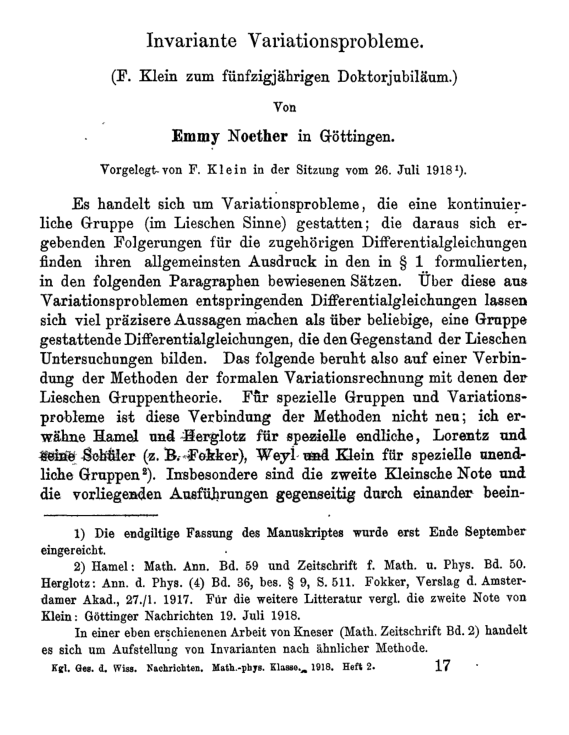
\includegraphics[height=0.52\textwidth,width=0.42\textwidth,viewport=0 0 450 580,clip]{Figures/Noether_theorem-1st_page.png}
\label{Noether_theorem}
\end{figure}
\begin{itemize}
\centering
	\item \textcolor{red}{能量守恒}~$\Longleftrightarrow$~\textcolor{magenta}{时间平移对称性}
	\item \textcolor{red}{动量守恒}~$\Longleftrightarrow$~\textcolor{magenta}{空间平移对称性}
	\item \textcolor{red}{角动量守恒}~$\Longleftrightarrow$~\textcolor{magenta}{空间旋转对称性}
\end{itemize}
}

\frame
{
	\frametitle{\textrm{驻波}}
\begin{figure}[h!]
\centering
\vspace{-15.5pt}
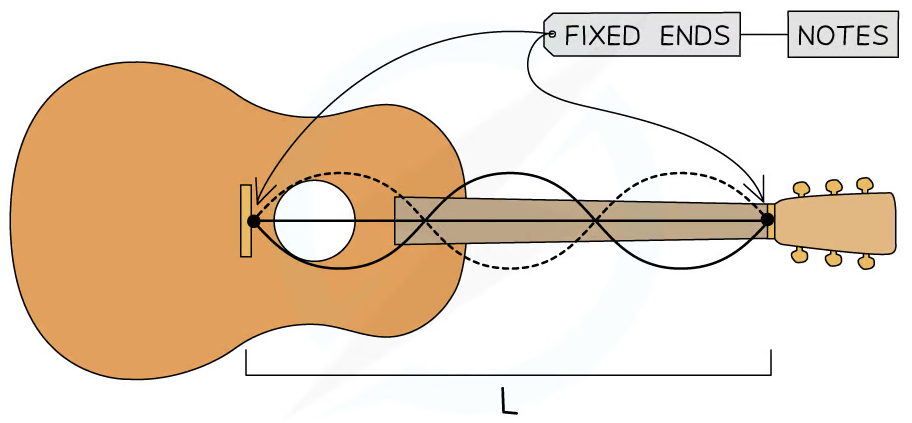
\includegraphics[height=0.40\textwidth,width=0.8\textwidth,viewport=0 0 900 450,clip]{Figures/Guitar-string.png}
\vskip 0.1pt
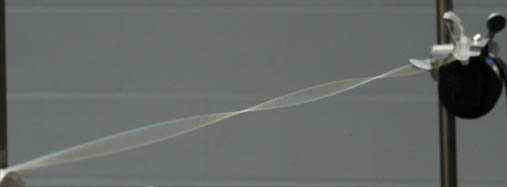
\includegraphics[height=0.35\textwidth,width=0.8\textwidth,viewport=0 0 122 48,clip]{Figures/string-standing-wave.jpg}
%\caption{\textrm{ABINIT}的Si.in}
\label{Standing_Wave_0}
\end{figure}
}

\frame
{
	\frametitle{驻波方程与势阱}
\begin{figure}[h!]
\centering
\vspace{-12.5pt}
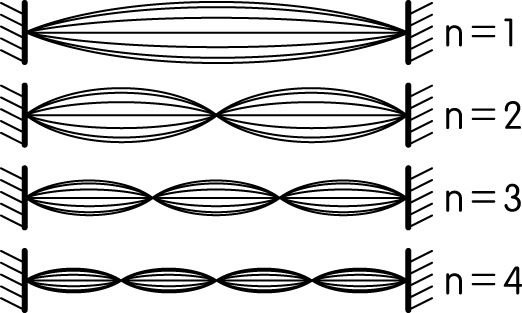
\includegraphics[height=0.32\textwidth,width=0.7\textwidth,viewport=0 0 125 75,clip]{Figures/Standing_wave.jpeg}
\vskip 2pt
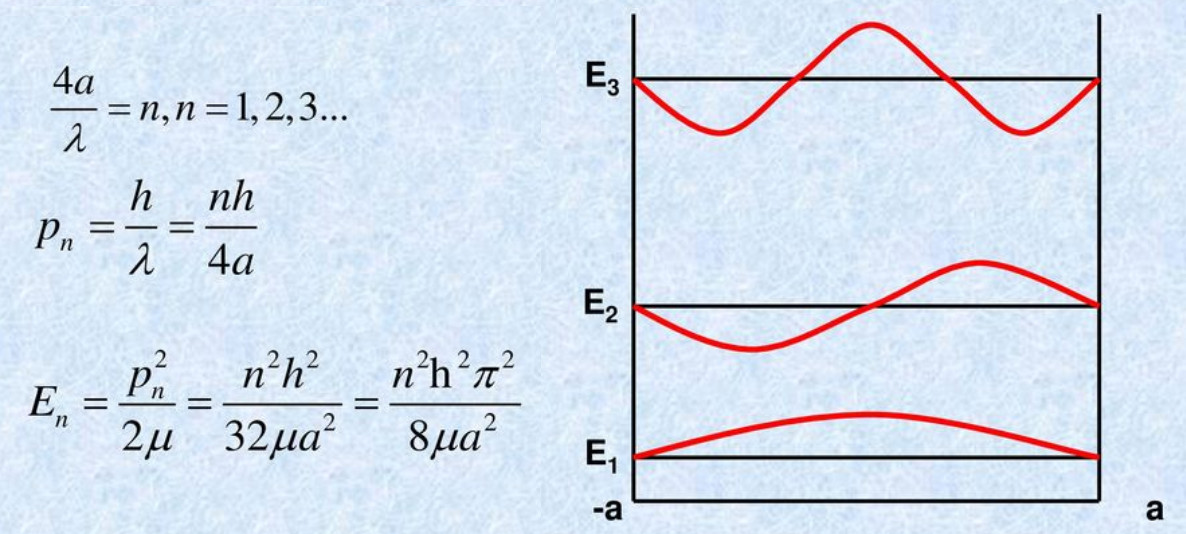
\includegraphics[height=0.40\textwidth,width=0.9\textwidth,viewport=0 0 1200 550,clip]{Figures/Standing_wave-energy.jpg}
%\caption{\textrm{ABINIT}的Si.in}
\label{Standing_Wave_1}
\end{figure}
}

\frame
{
	\frametitle{驻波方程与势阱}
\begin{figure}[h!]
\centering
\vspace{-5.5pt}
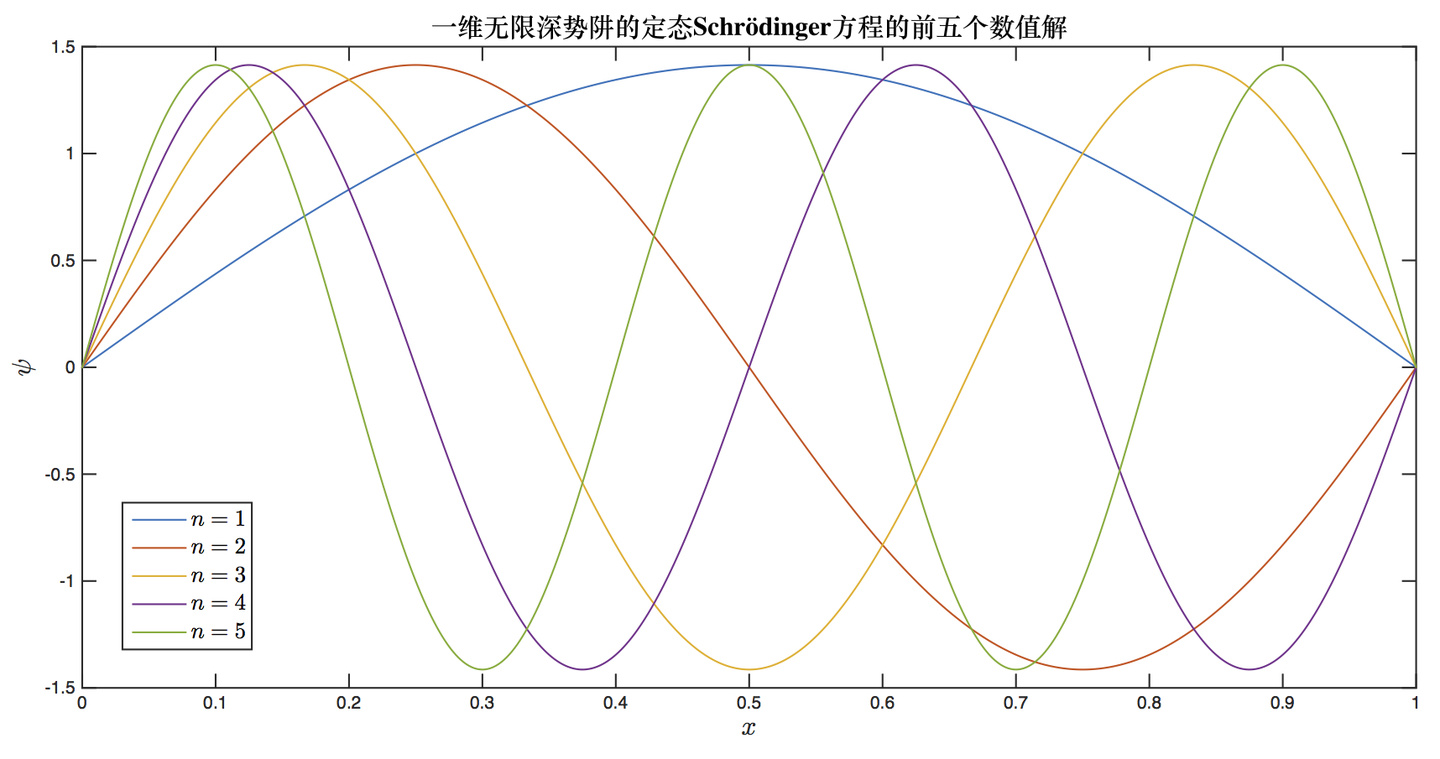
\includegraphics[height=0.55\textwidth,width=1.0\textwidth,viewport=0 0 720 400,clip]{Figures/Standing_wave-energy_1-5.jpg}
%\caption{\textrm{ABINIT}的Si.in}
\label{Standing_Wave_2}
\end{figure}
}

\frame
{
	\frametitle{驻波方程与势阱}
\begin{figure}[h!]
\centering
\vspace{-0.5pt}
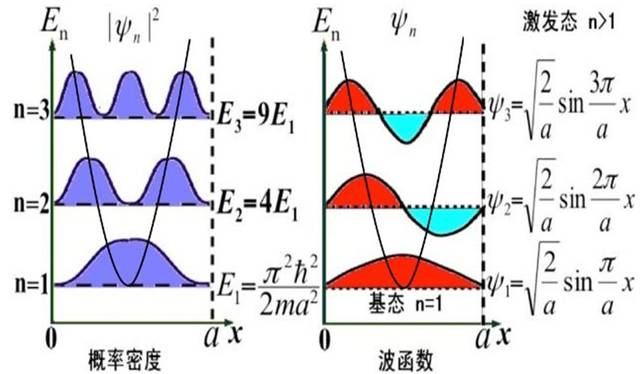
\includegraphics[height=0.46\textwidth,width=1.0\textwidth,viewport=0 0 650 390,clip]{Figures/Standing_wave_Energy.jpeg}
%\caption{\textrm{ABINIT}的Si.in}
\label{Standing_Wave_3}
\end{figure}
}

\frame
{
	\frametitle{原子中电子的驻波方程}
\begin{figure}[h!]
	\vspace{-10.5pt}
\centering
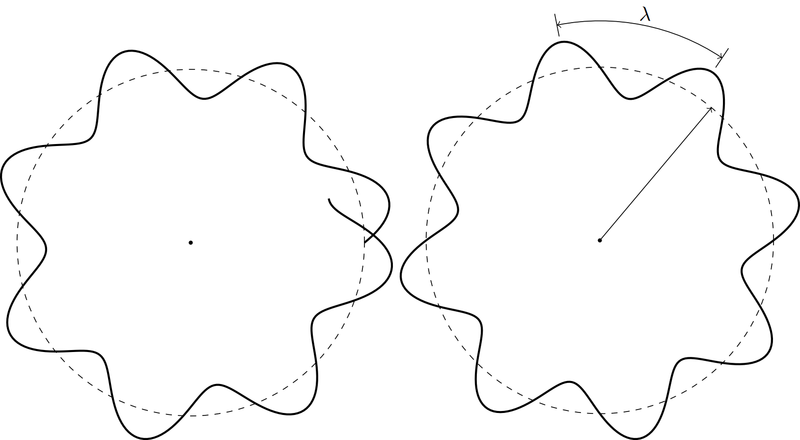
\includegraphics[height=0.38\textwidth,width=0.74\textwidth,viewport=0 0 840 440,clip]{Figures/Standing_wave-atom.png}
\vskip 2pt
\animategraphics[autoplay, loop, height=1.3in]{1}{Figures/Standing_wave_circle_}{1}{25}
\label{Atomic-electron_Standing_wave}
\end{figure}
}

\frame
{
	\frametitle{原子中的电子轨道和能量}
\begin{minipage}{0.43\textwidth}
\begin{figure}[h!]
%	\vspace{-14.8pt}
	\vspace{-4.8pt}
\centering
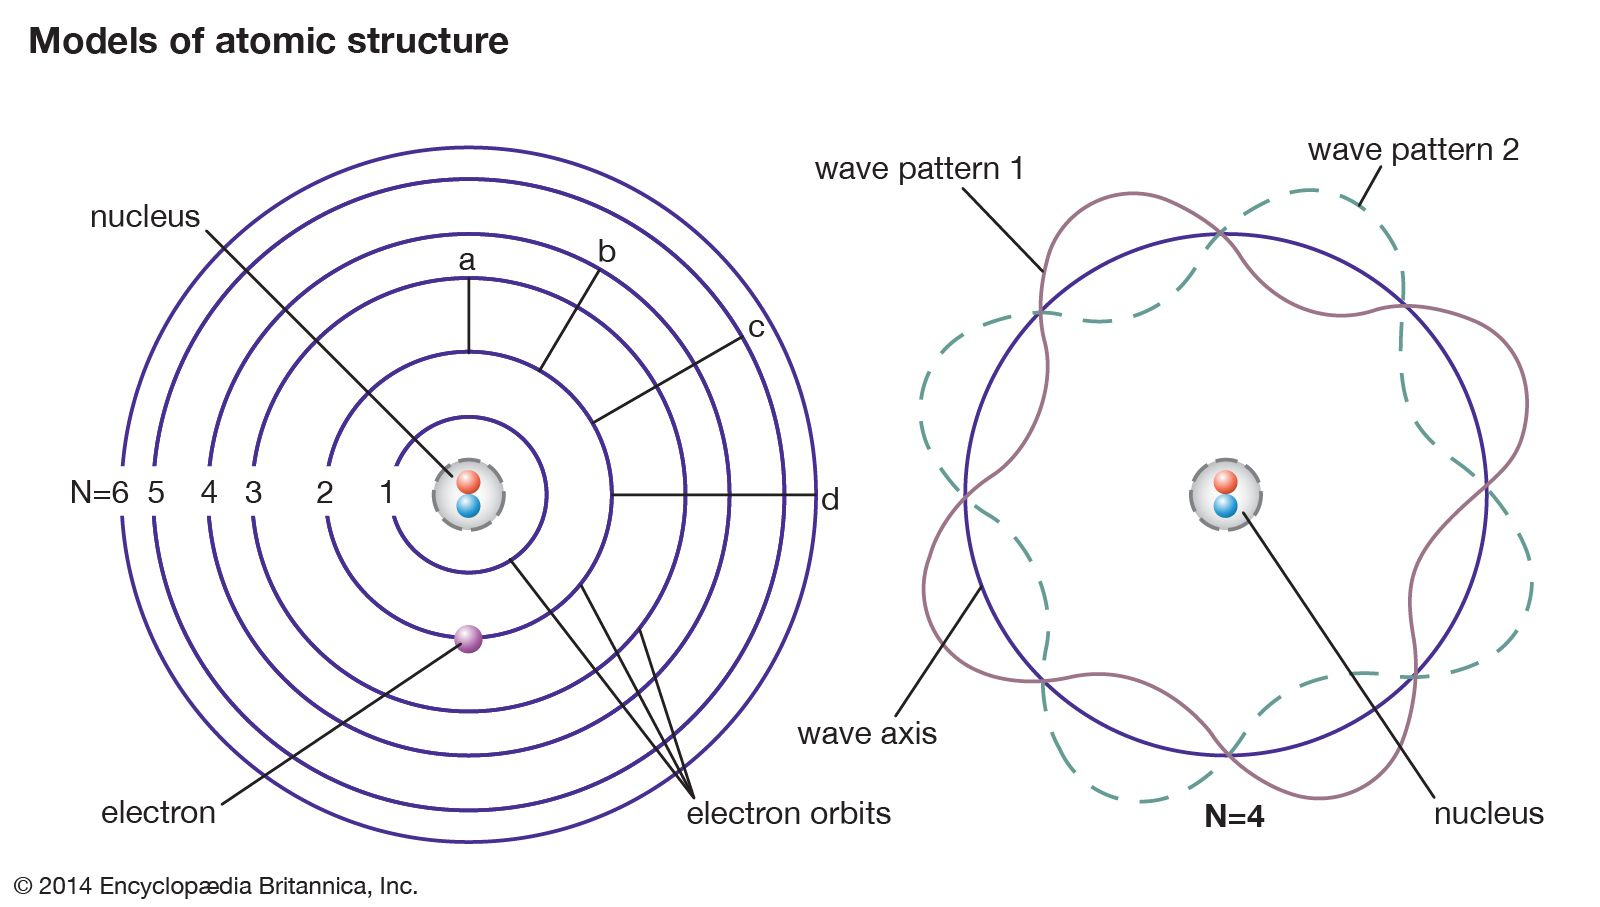
\includegraphics[height=0.57\textwidth,width=1.00\textwidth,viewport=0 50 1680 1000,clip]{Figures/electron-theory-Bohr-point-mass-energy-levels.jpg}
%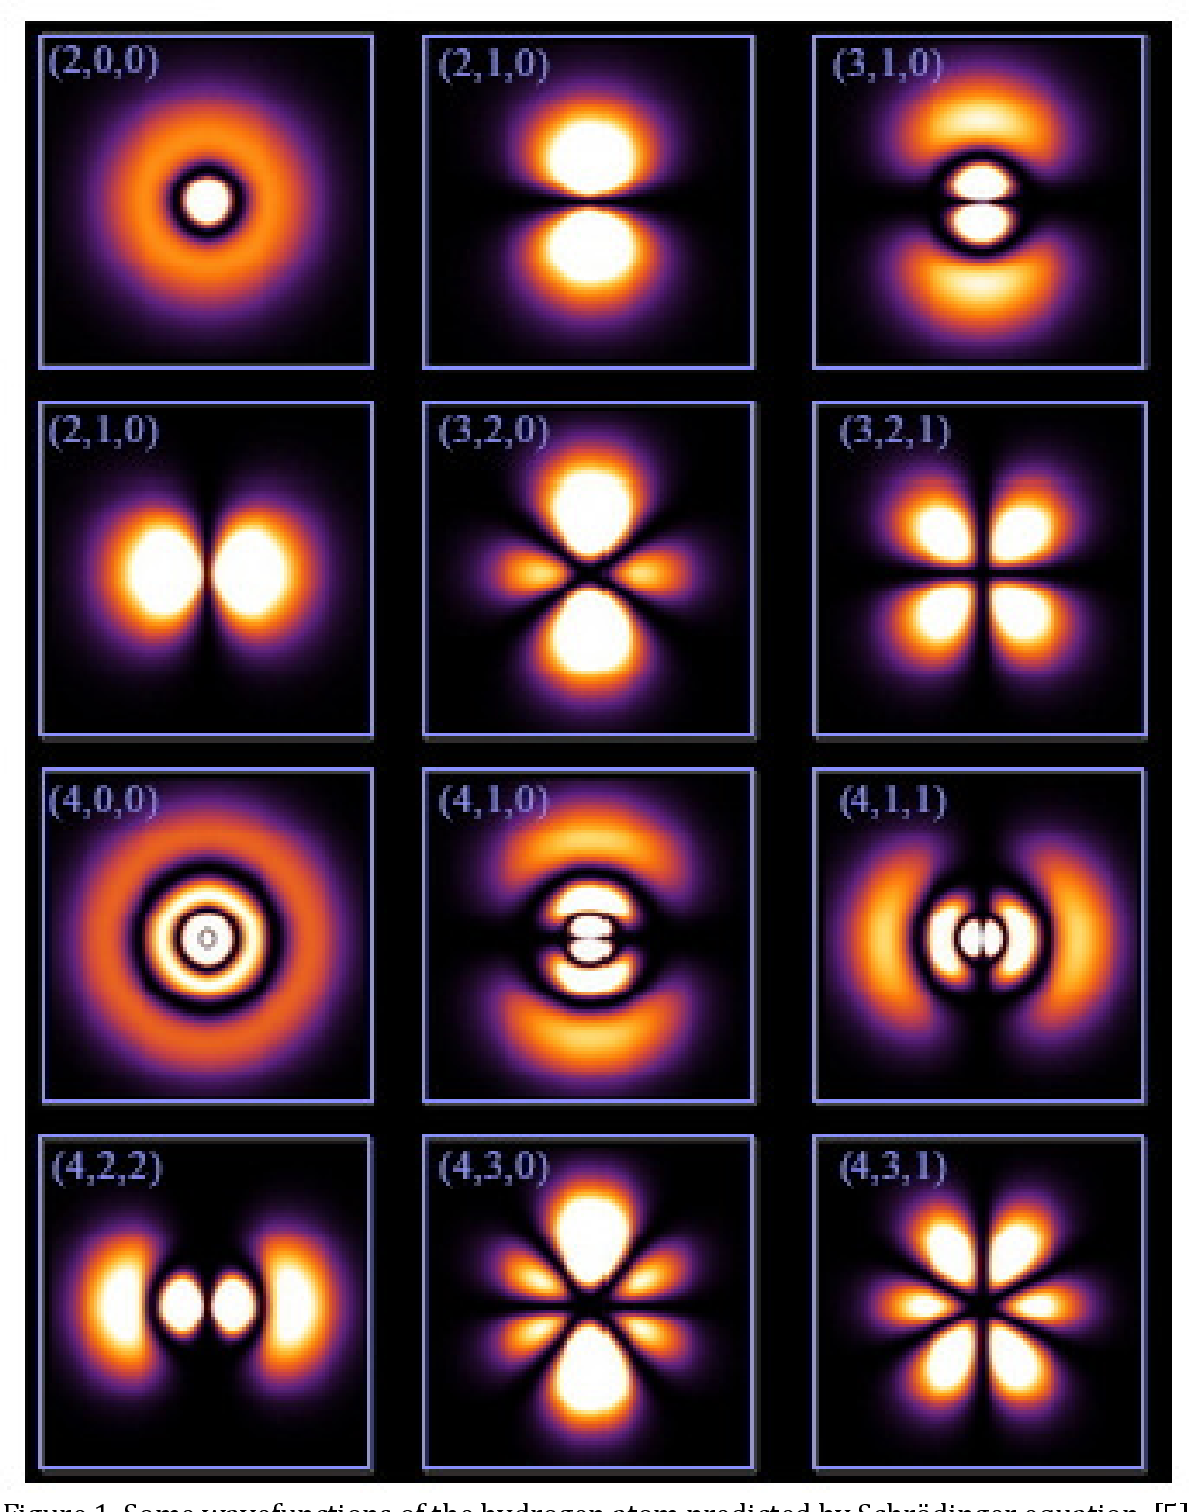
\includegraphics[height=1.23\textwidth,width=1.00\textwidth,viewport=0 10 1250 1500,clip]{Figures/wave_function.png}
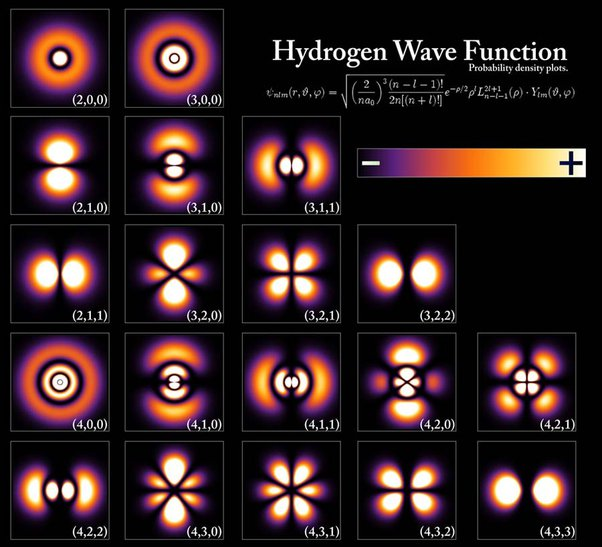
\includegraphics[height=0.95\textwidth,width=1.00\textwidth,viewport=0 0 630 650,clip]{Figures/wave_function-2.jpeg}
\label{Atomic-electron_wave}
\end{figure}
\end{minipage}
\begin{minipage}{0.55\textwidth}
\begin{figure}[h!]
	\vspace{-16.5pt}
\centering
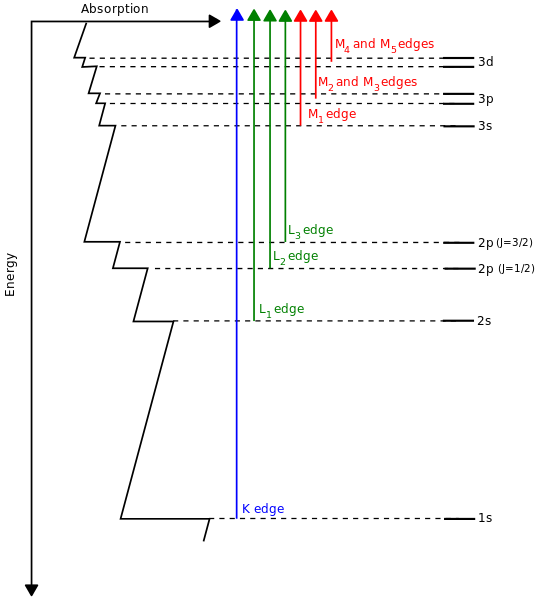
\includegraphics[height=1.10\textwidth,width=1.00\textwidth,viewport=0 0 560 600,clip]{Figures/Electron_orbital-energy.png}
\label{Atomic-electron_wave-energy}
\end{figure}
\end{minipage}
}

\frame
{
	\frametitle{\textrm{Schr\"odinger}~方程}
\begin{minipage}{0.49\textwidth}
\begin{figure}[h!]
\centering
%
\vspace{-25.5pt}
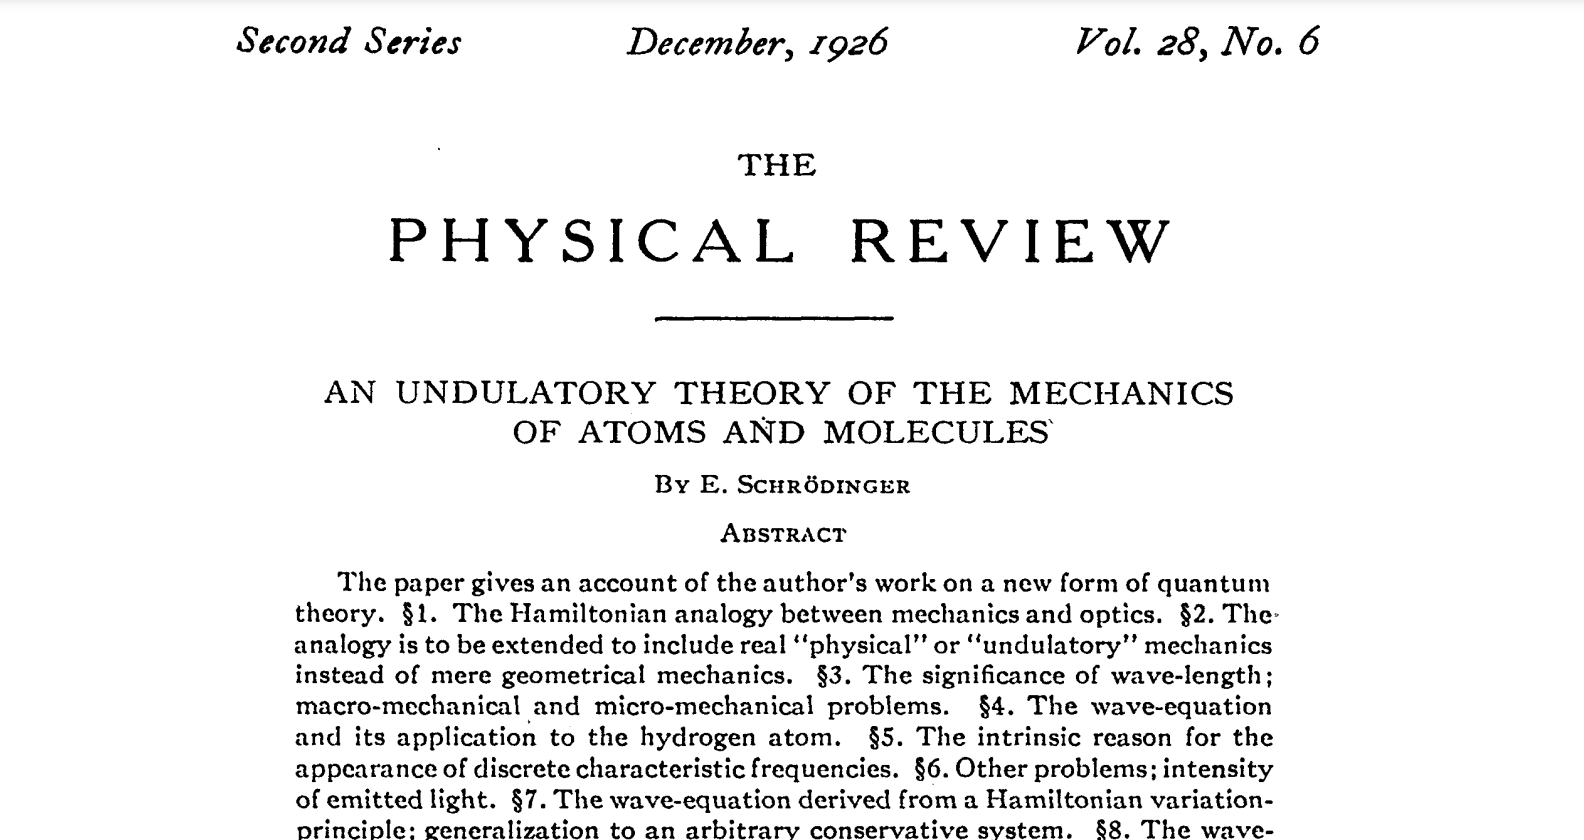
\includegraphics[height=1.80in,width=2.00in,viewport=180 0 1380 1100,clip]{Figures/Schrodinger_article.png}
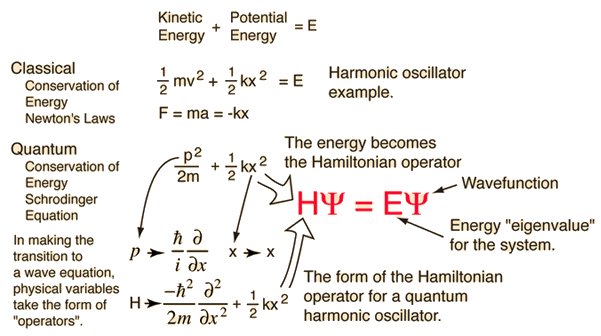
\includegraphics[height=1.20in,width=2.00in,viewport=0 0 600 350,clip]{Figures/Schrodinger_Equation.png}
\label{Schrodinger_Equation}
\end{figure}
\end{minipage}
\begin{minipage}{0.49\textwidth}
\begin{figure}[h!]
\centering
%
\vspace{-15.5pt}
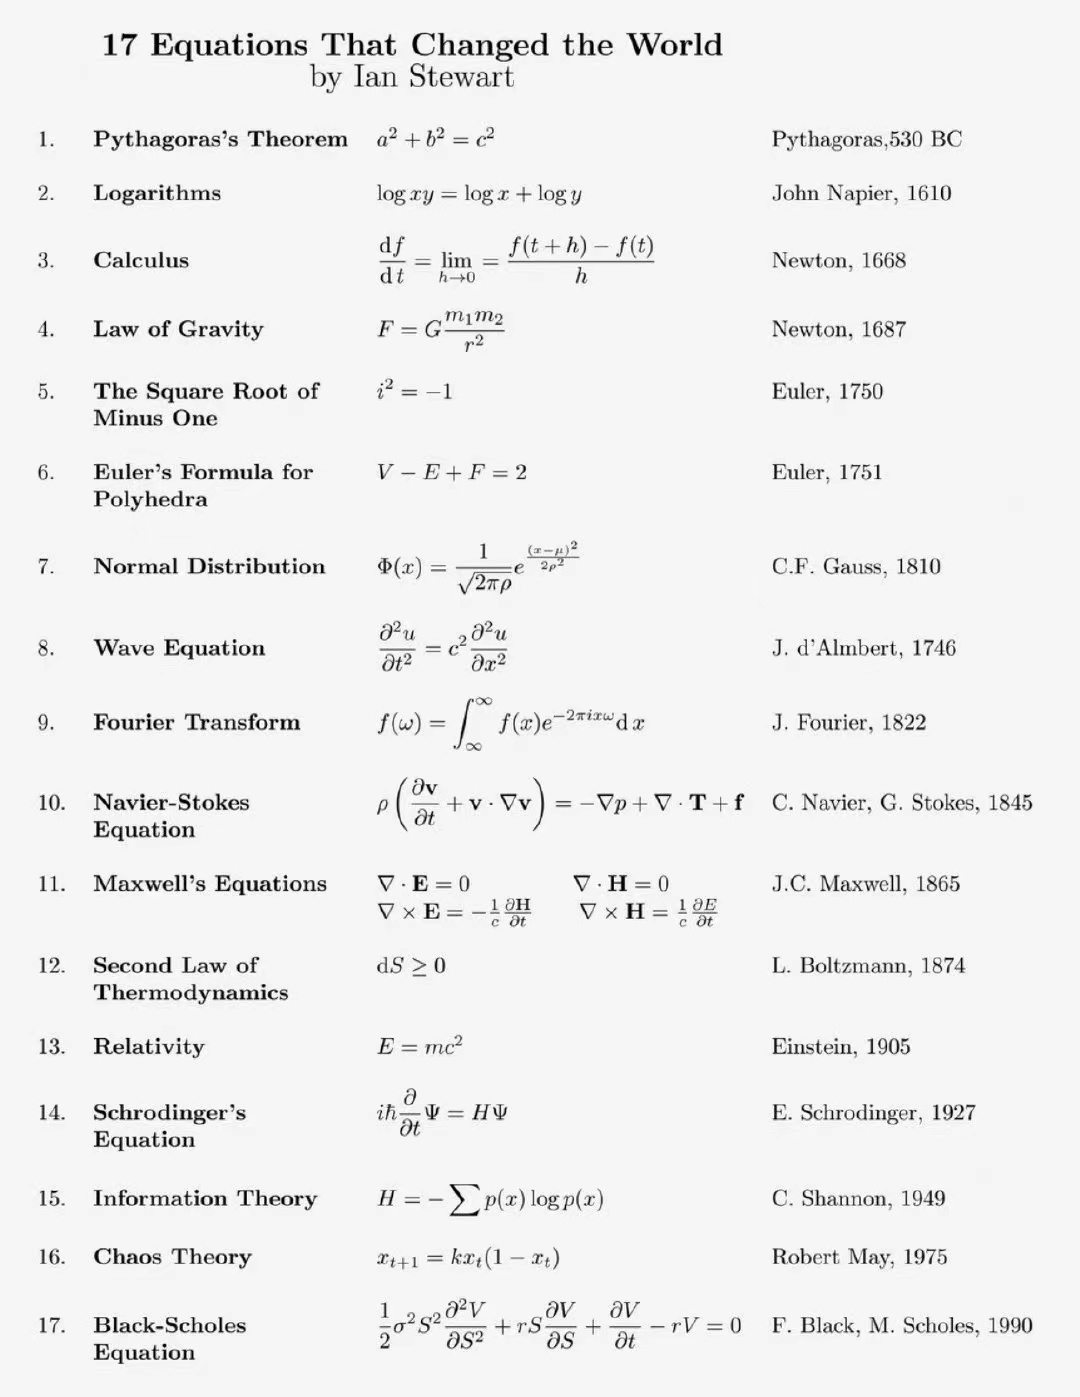
\includegraphics[height=2.85in,width=2.00in,viewport=0 0 780 1100,clip]{Figures/Great_Equation.jpg}
\label{Great_Equation}
\end{figure}
\end{minipage}
}

\frame
{
	\frametitle{量子力学的奠基人}
\begin{figure}[h!]
\centering
%\vspace{-25.5pt}
%\hspace*{-15.5pt}
%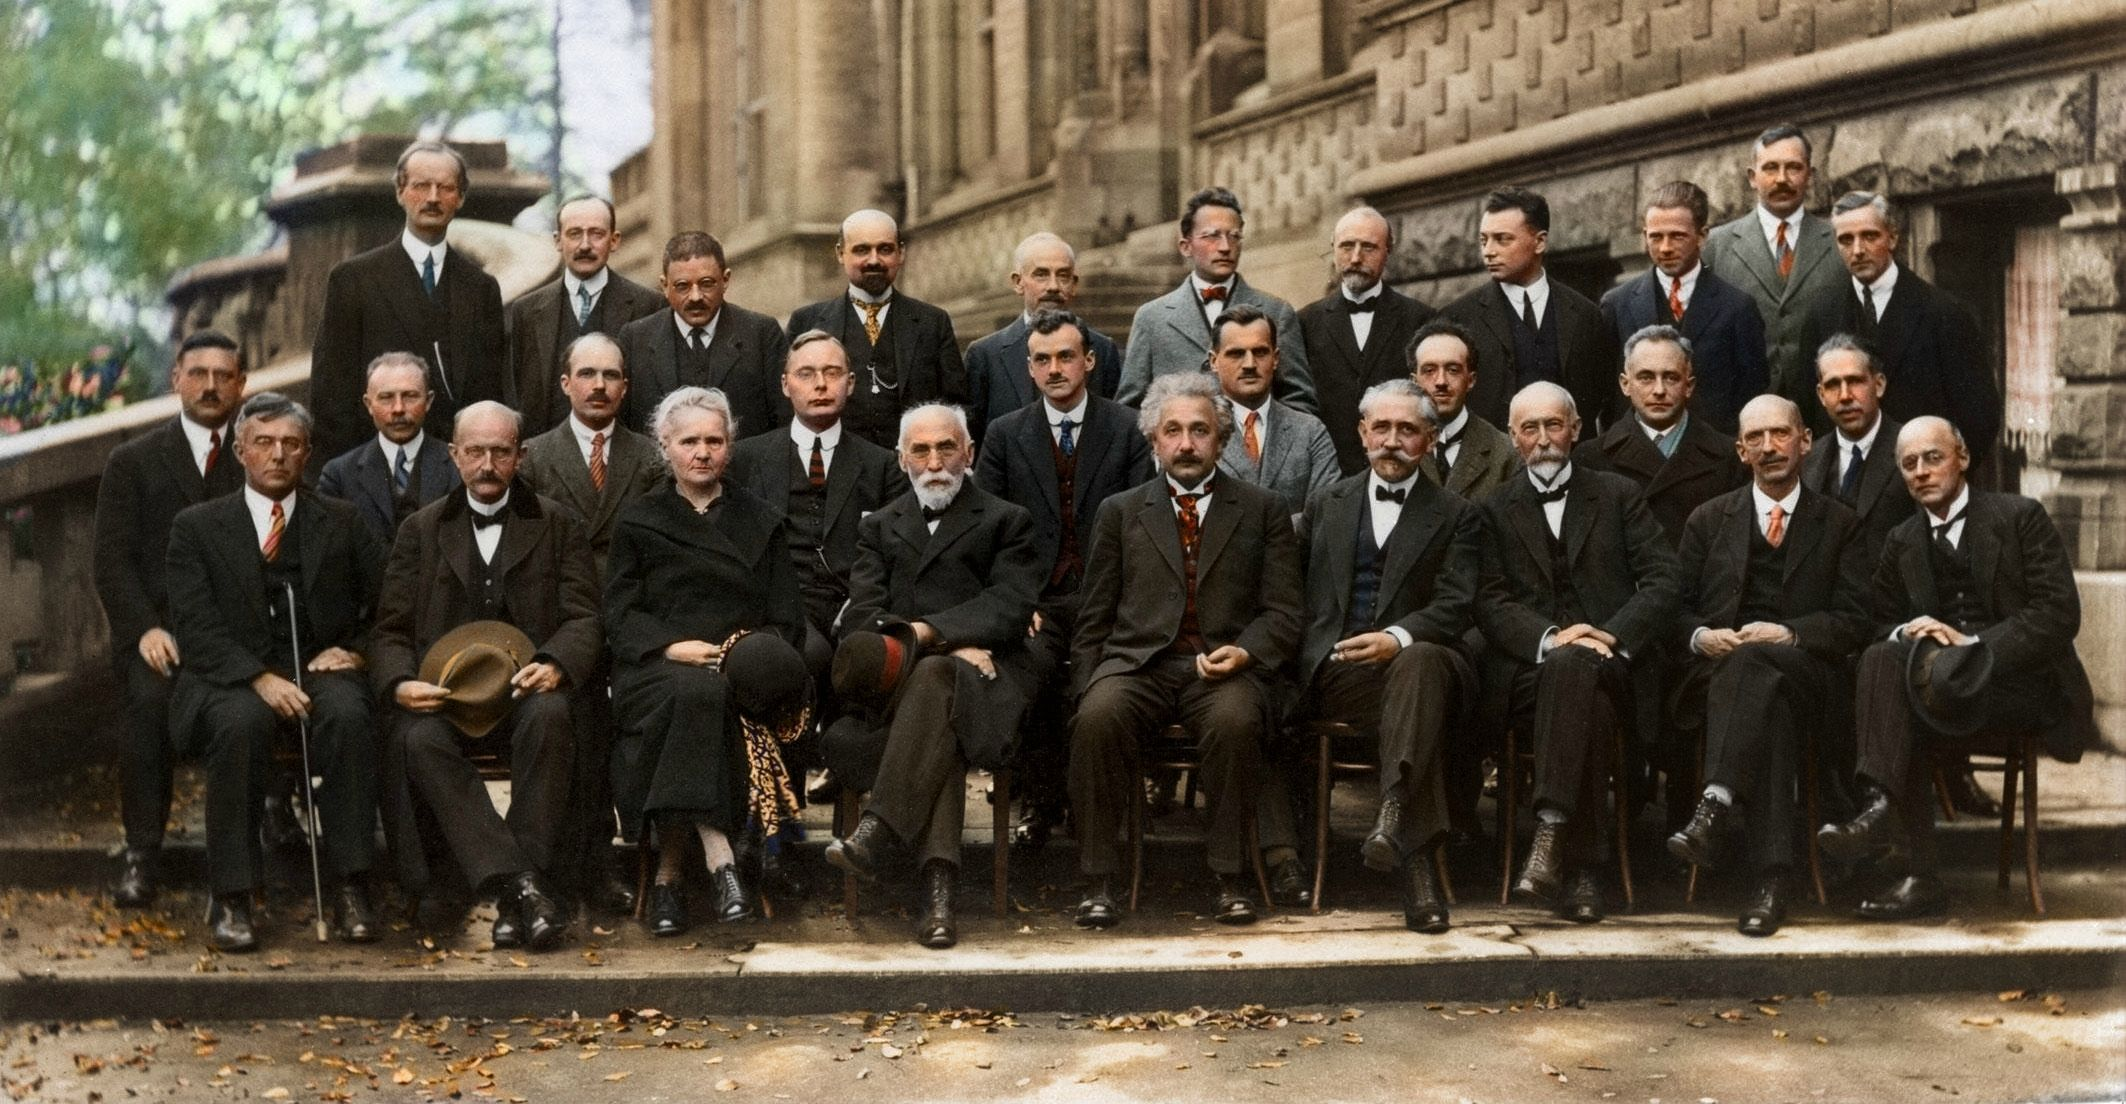
\includegraphics[height=0.57\textwidth,width=1.1\textwidth,viewport=0 0 2150 1050,clip]{Figures/Solvay_Conference-5-fine.jpg}
\vspace{-14.5pt}
\hspace*{-15.5pt}
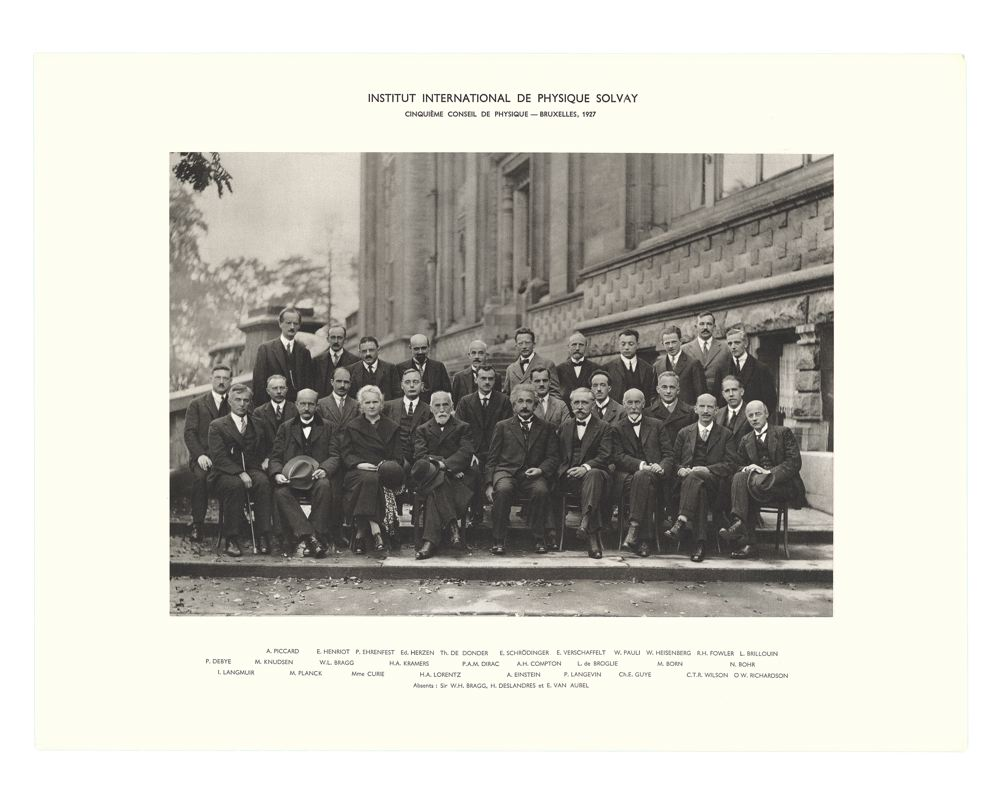
\includegraphics[height=0.50\textwidth,width=0.70\textwidth,viewport=150 105 850 710,clip]{Figures/Solvay_Conference-5.jpg}
\caption{\fontsize{7.5pt}{6.2pt}\selectfont{\textrm{The Fifth Solvay International Conference, Brussels, Belgium, Oct. 1927}}}
\label{Solvay Conference-5-fine}
\end{figure}
\vspace{-11.5pt}
\fontsize{4.1pt}{3.9pt}\selectfont{\textrm{\textcolor{blue}{前排左起}:~I.Langmuir(\textcolor{blue}{朗缪尔}) M.Planck(\textcolor{blue}{普朗克}) Marie Curie(\textcolor{blue}{居里夫人}) H.Lorentz(\textcolor{blue}{洛仑兹}) A.Einstein(\textcolor{blue}{爱因斯坦}) P.Langevin(\textcolor{blue}{朗之万}) Ch.E.Guye(\textcolor{blue}{古伊}) C.T.R.Wilson(\textcolor{blue}{威尔逊}) O.W.Richardson(\textcolor{blue}{理查森})\\
\textcolor{blue}{中排左起}:~P.Debye(\textcolor{blue}{德拜}) M.Knudsen(\textcolor{blue}{克努森}) W.L.Bragg(\textcolor{blue}{布拉格}) H.A.Kramers(\textcolor{blue}{克莱默}) P.A.M.Dirac(\textcolor{blue}{狄拉克}) A.H.Compton(\textcolor{blue}{康普顿}) L.de Broglie(\textcolor{blue}{德布罗意}) M.Born(\textcolor{blue}{玻恩}) N.Bohr(\textcolor{blue}{玻尔})\\
\textcolor{blue}{后排左起}:~A.Piccard(\textcolor{blue}{皮卡尔德}) E.Henriot(\textcolor{blue}{亨利厄特}) P.Ehrenfest(\textcolor{blue}{埃伦费斯特}) Ed.Herzen(\textcolor{blue}{赫尔岑}) Th.de Donder(\textcolor{blue}{德唐德}) E.Schr\"odinger(\textcolor{blue}{薛定谔}) E.Verschaffelt(\textcolor{blue}{费尔夏费尔特}) W.Pauli(\textcolor{blue}{泡利}) W.Heisenberg(\textcolor{blue}{海森堡}) R.H.Fowler(\textcolor{blue}{富勒}) L.Brillouin(\textcolor{blue}{布里渊})}}
}

\frame
{
	\frametitle{态叠加原理:~\textrm{Schr\"odinger's cat}}
\begin{figure}[h!]
\centering
\vspace{-10.5pt}
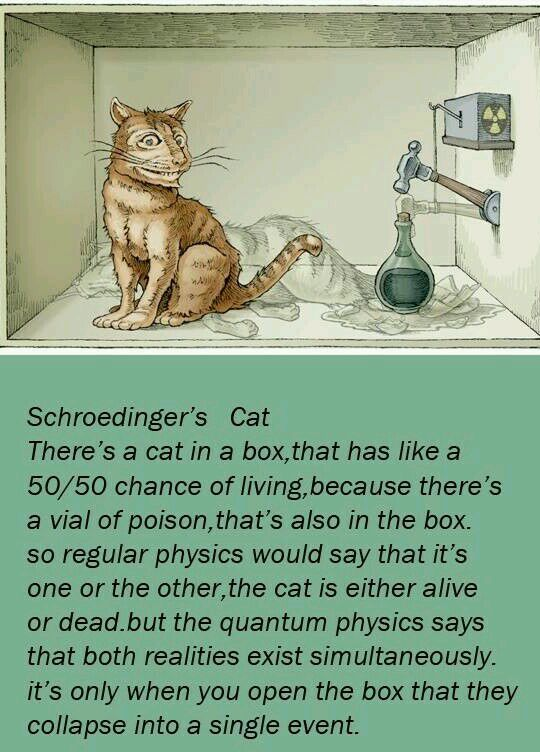
\includegraphics[height=0.70\textwidth,width=0.48\textwidth,viewport=0 0 550 750,clip]{Figures/Schrodinger-cat.jpg}
\includegraphics[height=0.70\textwidth,width=0.50\textwidth,viewport=0 0 720 930,clip]{Figures/Schrodinger_book.jpg}
%\caption{\textrm{ABINIT}的Si.in}
\label{Schrodinger-cat}
\end{figure}
}

\frame
{
	\frametitle{因果倒置:~\textrm{Delayed Choice Experiment}}
\begin{figure}[h!]
\centering
\vspace{-10.5pt}
\includegraphics[height=0.55\textwidth,width=1.0\textwidth,viewport=0 0 690 370,clip]{Figures/Schematic-diagram-of-delayed_choice-experiment.png}
\caption{\fontsize{5.2pt}{3.9pt}\selectfont{\textrm{Schematic diagram of Wheeler's delayed choice experiment with A Mach-Zehnder Interferometer.}}}
\label{Delayed_Choice-Experiment}
\end{figure}
}

\frame
{
	\frametitle{量子力学量力学}
\begin{figure}[h!]
\centering
\vspace{-13.5pt}
\includegraphics[height=0.75\textwidth,width=0.55\textwidth,viewport=0 0 500 650,clip]{Figures/Quote-Niels_Bohr-on-Quantum_mechanics.png}
\caption{\fontsize{5.2pt}{3.9pt}\selectfont{\textrm{A quote of Niels Bohr on Quantum mechanics.}}}
\label{Quote-Niels_Bohr}
\end{figure}
}

\frame
{
	\frametitle{几何原本:~公理体系的源头}
\begin{figure}[h!]
\centering
\vspace{-13pt}
\includegraphics[height=0.38\textwidth,width=0.65\textwidth,viewport=0 0 680 500,clip]{Figures/Element_Geometry_1.jpg}\\
\vspace{1pt}
\includegraphics[height=0.36\textwidth,width=0.65\textwidth,viewport=0 0 810 500,clip]{Figures/Element_Geometry_2.jpg}
%\caption{\textrm{ABINIT}的Si.in}
\label{Element_Geometru}
\end{figure}
}

\frame
{
	\frametitle{\textcolor{red}{公理体系}:~现代科学的逻辑起点}
\begin{figure}[h!]
\centering
\vspace{-10.5pt}
\includegraphics[height=0.68\textwidth,width=1.0\textwidth,viewport=0 0 770 500,clip]{Figures/Philp_Nature_Mach-2.png}
%\caption{\textrm{ABINIT}的Si.in}
\label{Philp_Nature}
\end{figure}
}

\frame[allowframebreaks]
{
	\frametitle{量子力学基本假设(\textcolor{red}{公理体系})}
	\begin{itemize}
		\item 全同粒子假设\\
			\textcolor{blue}{全同粒子组成的体系中,两个全同粒子相互调换不改变体系的状态}\\ 
			全同粒子是指\textcolor{red}{内禀性质完全相同的一类微观粒子}:\\例如,所有的电子是全同粒子 
		\item 波函数假设\\
			\textcolor{blue}{微观体系的运动状态可由波函数$\Psi$完全描述,波函数包含体系的所有性质}\\
			波函数$\Psi$一般要求满足\textcolor{red}{连续}、\textcolor{red}{有限}和\textcolor{red}{单值}三个条件
		\item 微观体系的运动状态\textcolor{blue}{波函数随时间变化的规律}:\\\textcolor{red}{遵从\textrm{Schr\"odinger}方程}
			$$\mathrm{i}\hbar\dfrac{\mathrm{d}}{\mathrm{d}t}|\Psi\rangle=\hat{\mathbf H}|\Psi\rangle$$
		\item 态叠加原理\\
			如果$\Psi_1$是体系的一个本征态,对应的本征值为$A_1$,$\Psi_2$也是体系的一个本征态,对应的本征值为$A_2$,则\textcolor{blue}{$$\Psi=C_1\Psi_1+C_2\Psi_2$$}\textcolor{red}{也是体系一个可能的存在状态}
		\item 力学量算符假设\\
			\textcolor{blue}{经典力学的物理量对应到量子力学中,要用线性~\textrm{Hermite}算符表示}(\textcolor{red}{\textrm{Hermite~}算符的本征函数构成完备空间})\\
			如动量算符 ~~~ $\hat{\mathbf{p}}=-\mathrm{i}\hbar\nabla$\\
			~~~位置算符 ~~~ $\hat{\mathbf r}=r$\\
			力学量算符之间有确定的对易关系(\textcolor{brown}{量子条件})
			$$[\hat{\mathbf F},\hat{\mathbf G}]=\hat{\mathbf F}\hat{\mathbf G}-\hat{\mathbf G}\hat{\mathbf F}$$ 
			
	\end{itemize}
}

\frame
{
	\frametitle{叠加态的数学表示:~矩阵}
\begin{figure}[h!]
\centering
\vspace{-1.5pt}
\hspace*{-0.12in}
\includegraphics[height=0.48\textwidth,width=1.05\textwidth]{Figures/Matrix_Rotation.png}
%\caption{\textrm{ABINIT}的Si.in}
\label{Matrix-Rotation}
\end{figure}
}

\frame
{
	\frametitle{量子化学学科创立}
	\begin{itemize}
		\item \textrm{1927}年,\textrm{\o.~Burrau}应用量子力学原理,完成\textrm{\ch{H2+}}离子的计算
		\item 同年,\textrm{Walter~Heitlery}和\textrm{Fritz~W.~London}对\textrm{\ch{H2}}分子的计算,标志着量子化学这一学科正式创立
	\end{itemize}
\begin{figure}[h!]
\centering
\vspace{-1.5pt}
\hspace*{-0.12in}
\includegraphics[height=0.48\textwidth,width=0.80\textwidth,viewport=0 10 260 175,clip]{Figures/Walter-Heitlery_Fritz-W-London.jpeg}
\caption{\textrm{W.~Heitlery (left) and F.~W.~London(right).}}
\label{Heitlery_London}
\end{figure}
}

%\frame
%{
%	\frametitle{\textrm{Paul Adrian Maurice Dirac's Commandments}}
%	\textrm{The underlying laws necessary for the mathematical treatment of a large part of physics \textcolor{red}{and the whole of chemistry} are thus completely known, and the difficulty lies only in the fact that application of these laws leads to equations that are \underline{too complex to be solved}.
%\vskip 15pt
%It therefore becomes desirable that approximation practical methods of applying quantum mechanics should be develop $\cdots$ 
%}

%\vskip 15pt
%\textrm{P.A.M Dirac Proc. Roy. Soc. Ser. A, \textbf{123}, 714, (1929)}
%}
%
\frame
{
%	\frametitle{\rm{Paul Dirac's Commandments\upcite{PRSLSA123-714_1929}}}
	\frametitle{\textrm{Paul Dirac's Commandments}}%\upcite{PRSLSA123-714_1929}}}
%	\textrm{\textcolor{purple}{The underlying laws necessary for the mathematical treatment of a large part of physics and the whole of chemistry are thus completely known, and the difficulty lies only in the fact that application of these laws leads to equations that are too complex to be solved.}}
\begin{figure}[h!]
\centering
\vspace{-10.5pt}
\includegraphics[height=0.71\textwidth,width=0.9\textwidth,viewport=0 0 1150 920,clip]{Figures/Dirac_comment.png}
%\caption{\textrm{ABINIT}的Si.in}
\label{Diract_Commandment}
\end{figure}
}

\frame
{
%	\frametitle{\textrm{DFT-SCF}}
\begin{figure}[h!]
\vspace*{-0.25in}
\centering
\includegraphics[height=2.80in,width=4.95in,viewport=5 3 1250 780,clip]{Figures/Method_Procedure.png}
%\caption{\tiny \textrm{Pseudopotential for metallic sodium, based on the empty core model and screened by the Thomas-Fermi dielectric function.}}%(与文献\cite{EPJB33-47_2003}图1对比)
\label{Method-Procedure}
\end{figure}
}

\frame
{
	\frametitle{王守竞先生与量子力学}
	王守竞(\textrm{Shou~Chin~Wang})的工作
	\begin{itemize}
		\item 计算氢分子的电子结构
			\vskip 2.5pt
			王守竞的论文\textcolor{purple}{《新量子力学下的常态氢分子问题》}%THE PROBLEM OF THE NORMAL HYDROGEN MOLECULE IN THE NEW QUANTUM MECHANICS
	\textcolor{blue}{
	\begin{displaymath}
		\Psi=C\left\{ \mathrm{exp}[-Z(r_1+ p_2)/a]+\mathrm{exp}[-Z( r_2+ p_1)/a] \right\}
	\end{displaymath}}
	{\fontsize{7.2pt}{6.5pt}\selectfont{其中$r_1$、$p_1$是第一个电子到两个原子核的距离,$r_2$,$p_2$是第二个电子到两个原子核的距离,$a$是\textrm{Bohr}半径}}\\
	得到的数值结果$Z=1.666$,$E_0=86.6\,\mathrm{kcal}$,$R_0=0.78$\,\textrm{\AA}
		\item 不对称陀螺(不对称转动)的能谱%On the Asymmetrical Top in Quantum Mechanics
			\vskip 2.5pt
			不对称陀螺的能级公式(\textcolor{purple}{“王氏公式”})
	\textcolor{blue}{
	\begin{displaymath}
		E= (hc8\pi)[Aj(j+1)+W]
	\end{displaymath}}
	\end{itemize}
}

\frame
{
	\frametitle{王守竞先生与量子力学}
\begin{figure}[h!]
\centering
\vspace{-10.5pt}
\includegraphics[height=0.66\textwidth,width=0.52\textwidth,viewport=0 0 270 350,clip]{Figures/Wang_Shoujing.jpg}
\caption{王守竞先生(1902-1984)}
\label{Wang_Shoujing}
\end{figure}
}

\frame
{
	\frametitle{王守竞先生与量子力学}
\begin{figure}[h!]
\centering
\vspace{-10.5pt}
\includegraphics[height=0.65\textwidth,width=1.0\textwidth,viewport=0 0 560 350,clip]{Figures/Collect_Wang.jpg}
\caption{\fontsize{7.2pt}{6.5pt}\selectfont{\textrm{左1:~王守竞,左2:~Ralph~Kronig 右1:~I.~I.~Rabi(1944年诺贝尔物理学奖获得者)}}}
\label{Collect_Wang}
\end{figure}
}

\section{密度泛函理论}       %Bookmark
\subsection{\rm{Thomas-Fermi~}模型}       %Bookmark
\frame
{
	\frametitle{\textrm{Thomas-Fermi}模型} 
	1927年,\textrm{Thomas}和\textrm{Fermi}基于均匀电子气模型上建立\textrm{Thomas-Fermi}模型,\textcolor{blue}{体系能量可用}\textcolor{red}{电子密度}\textcolor{blue}{表示}:
	\begin{itemize}
		\item 动能表达式
			$$T_{\mathrm{TF}}[\rho(\vec r)]=\dfrac3{10}(3\pi^2)^{\frac23}\int\rho^{\frac53}(\vec r)\mathrm{d}\vec r$$
		\item 外势$V_{ext}(\vec r)$下电子体系的能量泛函表达式为
			\begin{displaymath}
				\begin{aligned}
					E_{\mathrm{TF}}[\rho(\vec r)]=&\dfrac3{10}(3\pi^2)^{\frac23}\int\rho^{\frac53}(\vec r)\mathrm{d}\vec r\\
					&+\int\rho(\vec r)V_{ext}(\vec r)\mathrm{d}\vec r+\dfrac12\int\int\dfrac{\rho(\vec r_1)\rho(\vec r_2)}{|\vec r_2-\vec r_1|}\mathrm{d}\vec r_1\mathrm{d}\vec r_2
				\end{aligned}
			\end{displaymath}
		\item \textrm{Thomas-Fermi}模型完全没有考虑电子的交换-相关作用
	\end{itemize}
}

\frame
{
	\frametitle{\textrm{Thomas-Fermi-Dirac}模型} 
	1930年,\textrm{Dirac}将\textrm{Thomas-Fermi}模型修正,用局域密度近似考虑电子交换作用
			\begin{displaymath}
				\begin{aligned}
					E_{\mathrm{TFD}}[\rho(\vec r)]=&\dfrac3{10}(3\pi^2)^{\frac23}\int\rho^{\frac53}(\vec r)\mathrm{d}\vec r+\int\rho(\vec r)V_{ext}(\vec r)\mathrm{d}\vec r\\
					&+\dfrac12\int\int\dfrac{\rho(\vec r_1)\rho(\vec r_2)}{|\vec r_2-\vec r_1|}\mathrm{d}\vec r_1\mathrm{d}\vec r_2-\dfrac34\bigg(\dfrac3{\pi}\bigg)^{\frac13}\int\rho^{\frac43}(\vec r)\mathrm{d}\vec r
				\end{aligned}
			\end{displaymath}
			\begin{itemize}
				\item 在总电子数守恒约束条件
					$$\int\rho(\vec r)\mathrm{d}\vec r=N$$
					下,能量泛函$E_{\mathrm{TFD}}[\rho(\vec r)]$对密度$\rho(\vec r)$的变分极小获得体系的基态密度和基态能量
			\end{itemize}
}

\frame
{
	\frametitle{\textrm{Thomas-Fermi}模型}
	\begin{itemize}
		\item \textrm{Thomas-Fermi}模型用电子密度代替波函数描述问题是极大的简化,但模型过于粗糙:\\
%			\begin{enumerate}
%				\item 以均匀电子气的密度得到动能的表达式
%				\item 完全忽略电子间的交换-相关作用
%			\end{enumerate}
			不能正确描述相互作用电子体系的基本特征,如原子的壳层结构
		\item \textrm{Thomas-Fermi}模型虽不够精确,但可以通过引入修正项校正:
			\textrm{Dirac}交换泛函 $$E_X[\rho(\vec r)]=-\dfrac34\bigg(\dfrac3{\pi}\bigg)^{\frac13}\int\rho^{\frac43}(\vec r)\mathrm{d}\vec r$$
			\textrm{Wigner}相关泛函 $$E_C[\rho(\vec r)]=-0.056\int\dfrac{\rho^{\frac43}(\vec r)}{0.079+\rho^{\frac13}(\vec r)}\mathrm{d}\vec r$$
	\end{itemize}
	\textrm{Thomas-Fermi}模型为密度泛函理论\textrm{(DFT)}提供了重要的启示
}

\frame
{
	\frametitle{电荷密度代替电子}
\begin{figure}[h!]
\centering
\vspace{3.5pt}
\includegraphics[height=0.45\textwidth,width=1.0\textwidth,viewport=0 0 950 440,clip]{Figures/Schematic-illustration-of-transforming-many_electron-system-to-electron-density.png}
\caption{\fontsize{6.0pt}{4.5pt}\selectfont{\textrm{Schematic illustration of transforming many-electron system to electron density.}}}
\label{Density-Particle}
\end{figure}
}

\subsection{密度泛函理论}       %Bookmark
\frame                               %
{
\frametitle{密度泛函理论(\textrm{DFT})} %Slide Page Title
%   \secname
与传统的量子力学方法不同,密度泛函理论的基本变量是体系的基态电子密度。%通过体系的电子密度而非波函数确定体系的基态能量。
\begin{itemize}%[+-| alert@+>]
	\item 密度泛函理论的基石:\textrm{Hohenberg-Kohn}定理\upcite{PR136-B864_1964}
\vskip 5pt
\begin{itemize}%[+-| alert@+>]
   \setlength{\itemsep}{8pt}
 \item $E[\rho]=F_{\mathrm{HK}}[\rho]+\displaystyle\int\rho(\vec{r})v(\vec{r})\textrm{d}\vec{r}$ \\
\vskip 5pt 其中$F_{\mathrm{HK}}[\rho]=\underset{\Psi\to\rho}{\mathrm{Min}}\langle\Psi[\rho]|\hat{T}+\hat{W}|\Psi[\rho]\rangle$
是普适的泛函表达式。%,指明多电子体系的基态性质与基态密度间存在一一对应关系
     \textrm{\small{第一定理表明多电子体系的性质完全由体系的基态密度决定}}
   \item 如果$\tilde\Psi\neq\Psi$,
     $E[\tilde\rho]\geqslant E[\rho_0]$\\
     \textrm{\small{第二定理指出基态总能量泛函在体系基态电子密度处取极小值}}
   \end{itemize}
%\textrm{\small{第二定理指出基态总能量泛函在体系基态电子密度处取极小值}}
\vskip 8pt
 \item 密度泛函理论的优越性:用密度($\rho$)代替波函数($\Psi$)描述体系
\vskip 5pt
 \item 密度泛函理论的困难:能量密度泛函的精确形式未知
   \end{itemize}
}

\frame
{
	\frametitle{\rm{Creators of DFT}}
\begin{figure}[h!]
\vskip 10pt
\centering
\includegraphics[height=1.65in,width=4.0in,viewport=0 0 1562 610,clip]{Figures/Creators_of_DFT.png}
\caption{\tiny \textrm{Creators of DFT. Walter Kohn(left, in 1962) and his two postdoctoral fellows, Pierre Hohenberg (middle, in 1965) and Lujeu Sham (right).}}%(与文献\cite{EPJB33-47_2003}图1对比)
\label{Creator_of_DFT}
\end{figure}
}

\frame                               %
{
\frametitle{密度泛函理论(\textrm{DFT})}
\textrm{Kohn-Sham}方程\upcite{PR140-A1133_1965}:无相互作用体系+交换-相关能的贡献
$$(T_S+V_{e\!f\!f})|\varphi_i\rangle=\varepsilon_i|\varphi_i\rangle,\quad i=1,\cdots,N,\cdots$$
其中$T_S=-\dfrac12\nabla^2$~~是无相互作用体系的动能
\begin{displaymath}
	\begin{aligned}
		V_{e\!f\!f}(\vec r)=&V_{ext}(\vec r)+\displaystyle\int w(\vec r,\vec r\,')\rho(\vec r\,')\mathrm{d}\vec r\,'+V_{\mathrm{XC}}[\rho]\\
=&\displaystyle\int\dfrac{\rho(\vec r\,')}{|\vec r-\vec r^{\prime}|}\mathrm{d}\vec r\,'+V_{ext}(\vec r)+V_{\mathrm{XC}}[\rho]
	\end{aligned}
\end{displaymath}
$V_{ext}(\vec r)$是电子体系与外部的电荷或磁场相互作用\\
$V_{\mathrm{XC}}[\rho]=\dfrac{\delta E_{\mathrm{XC}}}{\delta\rho(\vec r)}$称为交换-相关势
\vskip 10pt
\textrm{Kohn-Sham}方程是形式上的单粒子方程
\vskip 6pt
\textrm{Kohn-Sham}方程的实质:\\\textcolor{red}{将动能泛函的主要部分分离出来,剩余部分放在交换-相关能中}
}

\frame{
\begin{figure}[h!]
\vskip -10pt
\centering
\includegraphics[height=2.65in,width=3.8in,viewport=0 0 362 275,clip]{Figures/DFT-particle-density.png}
\caption{\fontsize{6.0pt}{4.5pt}\selectfont{\textrm{Properties of a quantum mechanical system can be calculated by solving the SE (left). A more tractable, formally equivalent way is to solve the DFT KS equations (right).}}}%(与文献\cite{EPJB33-47_2003}图1对比)
\label{Schrodinger-equation-vs-Kohn-Sham-equation}
\end{figure}
}

\frame
{
	\frametitle{}
\begin{figure}[h!]
\centering
\includegraphics[height=2.65in,width=3.0in,viewport=0 0 600 570,clip]{Figures/Nobel_Prize_Chemistry_1998.png}
\caption{\tiny \textrm{The Nolbel Prize in Chemistry 1998 Summary.}}%(与文献\cite{EPJB33-47_2003}图1对比)
\label{Nobel_Prize_for_Chemistry}
\end{figure}
}

\frame
{
\frametitle{交换-相关能与交换-相关势}
实际考虑交换-相关能时,会将交换-相关能表示为交换能和相关能之和:
\begin{displaymath}
	E_{\mathrm{XC}}[\rho]=E_{\mathrm{X}}[\rho]+E_{\mathrm{C}}[\rho]=\int\varepsilon_{\mathrm{X}}[\rho]\rho(\vec{r}) \textrm{d}^3\vec{r}+\int\varepsilon_{\mathrm{C}}[\rho]\rho(\vec{r}) \textrm{d}^3\vec{r}
\end{displaymath}
$\varepsilon_{\mathrm{X}}[\rho]$和$\varepsilon_{\mathrm{C}}[\rho]$可理解为单电子的交换能和相关能
\vskip 20pt
交换-相关势通过交换-相关能计算得到:~
		\begin{displaymath}
			V_{\mathrm{XC}}^{\sigma}[\rho_{\alpha},\rho_{\beta}]=\dfrac{\delta E_{\mathrm{XC}}[\rho_{\alpha},\rho_{\beta}]}{\delta\rho_{\sigma}}=\dfrac{\delta\{E_{\mathrm{X}}[\rho_{\alpha},\rho_{\beta}]+E_{\mathrm{C}}[\rho_{\alpha},\rho_{\beta}]\}}{\delta\rho_{\sigma}}
		\end{displaymath}
		\textcolor{red}{注意}:~由于$E_{\mathrm{XC}}[\rho_{\sigma}]$对$\rho_{\sigma}$是非线性的\\
		\textcolor{blue}{$V_{\mathrm{XC}}=V_{\mathrm{X}}+V_{\mathrm{C}}$和$\varepsilon_{\mathrm{XC}}=\varepsilon_{\mathrm{X}}+\varepsilon_{\mathrm{C}}$不同,不要混淆这两个量}
}
%  \beamertemplateshadingbackground{blue!10}{yellow!10}

\frame                               %
{
\frametitle{交换-相关能密度泛函}
\textcolor{blue}{密度泛函理论的核心问题}:\\
\textrm{Kohn-Sham}方程用于实际计算,必须知道$E_{XC}[\rho]$或者$V_{XC}[\rho]$与$\rho(\vec r)$的泛函关系
\vskip 15pt
\begin{minipage}[b]{0.59\textwidth}
 \hspace*{-15pt}
 {\fontsize{7.5pt}{6.0pt}\selectfont\begin{itemize}%[+-| alert@+>]
	 \setlength{\itemsep}{10pt}
 \item \textrm{LDA}:泛函只与密度分布的局域值有关
 \item \textrm{GGA}:泛函依赖:局域密度及其梯度
 \item $meta$-\textrm{GGA}:泛函依赖的变量还有动能密度
 \item 杂化(\textrm{hybrid})泛函:泛函与占据轨道有关
 \item 其他的交换-相关能泛函
 \item<1-> 完全非局域泛函:理想泛函,不现实
 \end{itemize}}
\end{minipage}
\hfill
\begin{minipage}[b]{0.39\textwidth}
\hspace*{-10pt}
\includegraphics[height=1.7in,width=3.18in,viewport=10 5 1380 700,clip]{Figures/Jacobi-ladder.png}\\
\centering{\textcolor{red}{\textrm{\tiny Jacob's ladder}}}
\end{minipage}
% \begin{itemize}%[+-| alert@+>]
%\item 交换-相关能密度泛函
}

\frame                               %
{
	\frametitle{近似能量泛函$E_{\mathrm{XC}}[\rho]$的主要问题}
\vskip 20pt
\begin{enumerate}%[+-| alert@+>]
   \setlength{\itemsep}{10pt}
 \item  密度是整体变量:~电子自相互作用抵消不净\\%\quad\textrm{(LDA+U)}方法的校正%(\textrm{LDA+U})
	 用\textrm{DFT}计算电子数很少的体系,一般都会有较大的误差
 \item  电子相关:~简并和近简并基态的表示不合理\\
	 基态电子密度用不同的简并轨道计算时,体系能量应保持不变,但现有的近似能量泛函不具有这个性质
 \item  渐近行为:~处理弱相互作用体系的误差大\\
	 如\textrm{Van der Waals}相互作用和现有近似能量泛函本身的计算误差在同一量级
 \end{enumerate}
}

\frame                               %
{
	\frametitle{\textrm{Kohn-Sham}方程}
\begin{figure}[h!]
\centering
\vspace*{-0.21in}
\hspace*{-0.1in}
\includegraphics[height=2.7in,width=4.0in,viewport=2 5 1162 880,clip]{Figures/DFT.png}
\caption{\tiny \textrm{The Analysis of Kohn-Sham equation.}}%(与文献\cite{EPJB33-47_2003}图1对比)
\label{DFT}
\end{figure}
}

\subsection{常见泛函的一些形式}
\frame%[allowframebreaks]
{
	\frametitle{\rm{LDA}泛函}
	\begin{itemize}
		\item 交换能部分
	\begin{displaymath}
		\begin{aligned}
			\varepsilon_{\mathrm{X}}[\rho,\zeta]=&2^{-1/3}C_{\mathrm{X}}^{\sigma}g(\zeta)\rho^{1/3}(\vec r)\\
			E_{\mathrm{X}}[\rho,\zeta]=&\int\varepsilon_{\mathrm{X}}[\rho,\zeta]\rho(\vec r)\mathrm{d}\vec r\\
		\end{aligned}
	\end{displaymath}
	{\fontsize{7.5pt}{6.0pt}\selectfont{这里:~$C_{\mathrm{X}}^{\sigma}=\dfrac32\bigg(\dfrac3{4\pi}\bigg)^{1/3}$\\
		$g(\zeta)=\dfrac12\bigg[(1+\zeta)^{4/3}+(1-\zeta)^{4/3}\bigg]$\\
		$\zeta(\vec r)=\dfrac{[\rho_{\alpha}(\vec r)-\rho_{\beta}(\vec r)]}{[\rho_{\alpha}(\vec r)+\rho_{\beta}(\vec r)]}$}}
	\end{itemize}
}

\frame%[allowframebreaks]
{
	\frametitle{\rm{LDA}泛函}
	\begin{itemize}
		\item 相关能部分
			\begin{displaymath}
				\hspace*{-30pt}	\varepsilon_{\mathrm{C}}^{\mathrm{LDA}}(r_s,\zeta)=\varepsilon_{\mathrm{C}}(r_s,0)+a_{\mathrm{c}}(r_s)\dfrac{f(\zeta)}{f^{\prime\prime}(\zeta)}(1-\zeta^4)+[\varepsilon_{\mathrm{c}}(r_s,1)-\varepsilon_{\mathrm{c}}(r_s,0)]f(\zeta)\zeta^4
			\end{displaymath}
			{\fontsize{7.5pt}{6.0pt}\selectfont{这里:~$r_s=\bigg[\dfrac3{4\pi}(\rho_{\alpha}+\rho_{\beta})^{-1}\bigg]^{1/3}$~$f(\zeta)=[(1+\zeta)^{4/3}+(1-\zeta)^{4/3}-2]/(2^{4/3}-2)$\\
			$\varepsilon_{\mathrm{C}(r_s,0)}$、$\varepsilon_{\mathrm{C}(r_s,1)}$、$a_{\mathrm{C}(r_s)}$由经验公式
			\begin{displaymath}
				\begin{aligned}
					&G(r_s,A,\alpha_1,\beta_1,\beta_2+\beta_3+\beta_4)\\
					=&-2A(1+\alpha_1r_s)\ln\bigg[1+\dfrac1{2A(\beta_1r_s^{1/2}+\beta_2r_s+\beta_2r_s^{3/2}+\beta_1r_s^2)}\bigg]
				\end{aligned}
			\end{displaymath}
		计算。其中$A$、$\alpha_1$、$\beta_1$、$\beta_2$、$\beta_3$、$\beta_4$是参数,通过拟合实验结果确定}}
		\begin{displaymath}
			E_{\mathrm{C}}[\rho]=\int\rho(\vec r)\varepsilon_{\mathrm{C}}(\vec r)\mathrm{d}\vec r
		\end{displaymath}
	\end{itemize}
}

\frame%[allowframebreaks]
{
	\frametitle{\rm{GGA}泛函}
	\begin{itemize}
		\item 交换能泛函:
			\begin{itemize}
				\item \textrm{PW91}
					\begin{displaymath}
						\begin{aligned}
							E_{\mathrm{X}}^{\mathrm{PW91}}[\rho_{\alpha},\rho_{\beta}]=&\dfrac12(E_{\mathrm{X}}^{\mathrm{PW91}}[2\rho_{\alpha}]+E_{\mathrm{X}}^{\mathrm{PW91}}[2\rho_{\beta}])\\
							E_{\mathrm{X}}^{\mathrm{PW91}}[\rho]=&-\dfrac34\bigg(\dfrac3\pi\bigg)^{1/3}\int\rho^{4/3}(\vec r)F(x)\mathrm{d}\vec r
						\end{aligned}
					\end{displaymath}
					\hspace*{-30 pt}{\fontsize{4.5pt}{4.0pt}\selectfont{这里:~$F(x)=\dfrac{1+0.19645(hx)\sinh^{-1}(7.7956hx)+(hx)^2\{0.2743-0.1508\mathrm{exp}[-100(hx)^2]\}}{1+0.19645(hx)\sinh^{-1}(7.7956hx)+0.004(hx)^4}$}\\
					$h=(24\pi^2)^{-1/3}$,~~~$x=|\nabla\rho|\rho^{-4/3}$}
				\item \textrm{PBE}
			\begin{displaymath}
				E_{\mathrm{X}}^{\mathrm{PBE}}[\rho,x]=E_{\mathrm{X}}^{\mathrm{LDA}}[\rho,x]-C_{\mathrm{X}}\int a\bigg(1-\dfrac1{bx^2}\bigg)\rho^{4/3}(\vec r)\mathrm{d}\vec r
			\end{displaymath}
			{\fontsize{4.5pt}{4.0pt}\selectfont{其中:~$C_{\mathrm{X}}=\dfrac34\bigg(\dfrac3\pi\bigg)^{1/3}$\\$a=0.804$,~~~$b=0.273$~是非经验参数}}
			\end{itemize}
	\end{itemize}
}

\frame%[allowframebreaks]
{
	\frametitle{\rm{GGA}泛函}
	\begin{itemize}
		\item 相关能泛函:
			\begin{itemize}
				\item \textrm{PW91}
					\begin{displaymath}
						\begin{aligned}
							E_{\mathrm{C}}^{\mathrm{PW91}}[\rho_{\alpha},\rho_{\beta}]=&\int\mathrm{d}\vec r\rho(\vec r)[\varepsilon_{\mathrm{C}}^{\mathrm{LSDA}}(r_s,\zeta)]+H(t,r_s,\zeta)\\
							H=&H_0+H_1
						\end{aligned}
					\end{displaymath}
					{\fontsize{4.5pt}{4.0pt}\selectfont{这里:~
						\begin{displaymath}
							\begin{aligned}
								H_0=&f^3(\zeta)\dfrac{\beta^2}{2\alpha}\ln\bigg(1+\dfrac{2\alpha}{\beta}\dfrac{t^2+At^4}{1+At^2+A^2t^4}\bigg)\\
								A=&\dfrac{2\alpha}{\beta}\dfrac1{\mathrm{exp[-2\alpha\varepsilon_{\mathrm{C}}^{\mathrm{LDA}}(r_s,\zeta)}/f^3(\zeta)\beta^2]-1}\\
							t=&\dfrac{|\nabla\rho|}{2f(\zeta)k_s\rho}~~~f(\zeta)=\dfrac12\bigg[(1+\zeta)^{2/3}+(1-\zeta)^{2/3}\bigg]\\
							k_s=&[4(3\pi^{-1}\rho)^{1/3}]^{1/2}
							\end{aligned}
						\end{displaymath}
						参数 $\alpha=0.09$,~~~$\beta=\nu C_{\mathrm{C}}(0)$\\
						$\nu=(16/\pi)(3\pi^2)^{1/3}$,~~~$C_{\mathrm{C}}(0)=0.004235$
				}}
			\end{itemize}
	\end{itemize}
}

\frame%[allowframebreaks]
{
	\frametitle{\rm{meta-GGA}泛函}
	\begin{itemize}
		\item 交换能泛函
			\begin{itemize}
				\item \textrm{TPSS}
					\begin{displaymath}
						\begin{aligned}
							E_{\mathrm{X}}^{\mathrm{TPSS}}[\rho]&=\int\mathrm{d}\vec r\rho(\vec r)\varepsilon_{\mathrm{X}}^{\mathrm{LSDA}}(\vec r)F_{\mathrm{X}}^{\mathrm{TPSS}}(p,z)\\
							F_{\mathrm{X}}^{\mathrm{TPSS}}&=1+\kappa-\dfrac{\kappa}{1+x/\kappa}
						\end{aligned}
					\end{displaymath}
{\fontsize{4.5pt}{4.0pt}\selectfont{这里:~
	$\rho(\vec r)=\rho_{\alpha}(\vec r)+\rho_{\beta}({\vec r})$,~~~$\varepsilon_{\mathrm{X}}^{\mathrm{LSDA}}(\vec r)=-\dfrac3{4\pi}[3\pi^2\rho(\vec r)]^{1/3}$
\\
\begin{displaymath}
	\begin{aligned}
		x=&\left\{\bigg[\dfrac{10}{81}+\dfrac{cz^2}{(1+z^2)^2}\bigg]p+\dfrac{146}{2025}\bar{q}_b^2-\dfrac{73}{405}\bar{q}_b\bigg[\dfrac12\bigg(\dfrac35z\bigg)^2+\dfrac12p^2\bigg]^{1/2}\right.\\
		&+\left.\dfrac1{\kappa}\bigg(\dfrac{10}{81}\bigg)^2p^2\dfrac{20e^{1/2}}{81}\bigg(\dfrac35z\bigg)^2+e\mu p^3\right\}(1+e^{1/2}p)^{-2}\\
		p=&\dfrac{|\nabla\rho(\vec r)|^2}{4(3\pi^2)^{2/3}\rho^{8/3}(\vec r)}, ~~~ \bar{q}_b=\dfrac{(9/20)(\alpha-1)}{[1+b\alpha(\alpha-1)]^{1/2}}+2p/3
	\end{aligned}
\end{displaymath}
$z=\tau_w/\tau$,~~~$\tau_w=\dfrac{|\nabla\rho(\vec r)|^2}{8\rho(\vec r)}$,~~~$\tau=\sum\limits_{\sigma}\tau_{\sigma}$\\
$\alpha=(\tau-\tau_w)/\tau_{\mathrm{unif}}=(5p/3)(z^{-1}-1)$,~~~$\tau_{\mathrm{tiff}}=\dfrac3{10}(3\pi^2)^{2/3}[\rho(\vec r)]^{5/3}$
}}
			\end{itemize}
	\end{itemize}
}


\frame%[allowframebreaks]
{
	\frametitle{\rm{meta-GGA}泛函}
	\begin{itemize}
		\item 相关能泛函
			\begin{itemize}
				\item {\textrm{TPSS}}
					\begin{displaymath}
						E_{\mathrm{C}}^{\mathrm{TPSS}}[\rho_{\alpha,\rho_{\beta}}]=\int\mathrm{d}\vec r\rho(\vec r)\varepsilon_{\mathrm{C}}^{\mathrm{TPSS0}}[1+\mathrm{d}\varepsilon_{\mathrm{C}}^{\mathrm{TPSS0}}(\tau_w/\tau)^3]
					\end{displaymath}
{\fontsize{4.5pt}{4.0pt}\selectfont{这里:~
	\begin{displaymath}
		\begin{aligned}
			\varepsilon_{\mathrm{C}}^{\mathrm{TPSS0}}=&\varepsilon_{\mathrm{C}}^{\mathrm{PBE}}(\rho_{\alpha},\rho_{\beta},\nabla\rho_{\alpha},\nabla\rho_{\beta})[1+C(\zeta,\xi)(\tau_w/\tau)^2]\\
			&-\bigg[1+C(\zeta,\xi)(\tau_w/\tau)^2\sum\limits_{\sigma}\dfrac{\rho_{\sigma}(\vec r)}{\rho(\vec r)}\bar{\varepsilon}_{\mathrm{C}}\bigg]\\
			\bar{\varepsilon}_{\mathrm{C}}=&\max[\varepsilon_{\mathrm{C}}^{\mathrm{PBE}}(\rho_{\alpha},0,\nabla\rho_{\alpha},0),\varepsilon_{\mathrm{C}}^{\mathrm{PBE}}(\rho_{\alpha},\rho_{\beta},\nabla\rho_{\alpha},\nabla\rho_{\beta})]\\
			C(\zeta,\xi)=&\dfrac{C(\zeta,0)}{\{1+\xi^2[(1+\zeta)^{-4/3}+(1-\zeta)^{-4/3}]/2\}^4}
		\end{aligned}
	\end{displaymath}
	$\xi=\dfrac{|\nabla\zeta|}{2[3\pi^2\rho(\vec r)]^{1/3}}$, ~~~$C(\zeta,0)=0.53+0.87\zeta^2+0.50\zeta^4+2.26\zeta^6$
}}
			\end{itemize}
	\end{itemize}
	\vskip 5pt
	\textrm{TPSS}泛函的特点:~\\
	\vskip 3pt
	{\fontsize{7.5pt}{6.0pt}\selectfont{不包含依靠实验数据的可调参数,数字系数由精确能量泛函满足的条件确定\\
		\textcolor{blue}{对电子分布较为均匀的晶体体系和电子分布激烈变化的分子体系都有较高的精度} }}
}

\frame
{
	\frametitle{\rm{hybrid}泛函}
	体系\textrm{Hamilton}算符表示为
	\begin{displaymath}
		\hat{H}_{\lambda}=-\dfrac12\sum_i^N\nabla^2+\sum_i^NV_i(\rho,\lambda)+\dfrac{\lambda}2\sum_i^N\sum_{j(j\neq i)}^N\dfrac1{r_{ij}}
	\end{displaymath}
	\begin{displaymath}
		\mbox{\textcolor{blue}{$\lambda$表征电子间相互作用程度}}\left\{
		\begin{aligned}
			&\lambda=0:~\mbox{无相互作用的参考体系}\\
			&\lambda=1:~\mbox{存在相互作用的真实体系}
		\end{aligned}
		\right.
	\end{displaymath}
	交换-相关能表示为
	\begin{displaymath}
		\begin{aligned}
			E_{\mathrm{XC}}^{\lambda}=&\dfrac12\int\mathrm{d}\vec r_1\rho_1^{\lambda}(\vec r_1)\int\dfrac{h_{\mathrm{XC}}^{\lambda}(\vec r_1,\vec r_2)}{\vec r_1-\vec r_2}\mathrm{d}\vec r_2\\
			E_{\mathrm{XC}}=&\int E_{\mathrm{XC}}^{\lambda}\mathrm{d}\lambda
		\end{aligned}
	\end{displaymath}
	{\fontsize{4.5pt}{4.0pt}\selectfont{这里:~$h_{\mathrm{XC}}(\vec r_1,\vec r_2)=\dfrac{2\rho_2(\vec r_1,\vec r_2)}{\rho(\vec r_1)}-\rho_1(\vec r_2)$}}
}

\frame
{
	\frametitle{\rm{hybrid}泛函}
	\begin{itemize}
		\item \textrm{half-to-half}
			\begin{displaymath}
				\begin{aligned}
					E_{\mathrm{XC}}=&\dfrac12(E_{\mathrm{XC}}^0+E_{\mathrm{XC}}^1)=\dfrac12E_{\mathrm{XC}}^{\mathrm{Exact}}+\dfrac12E_{\mathrm{XC}}^1\\
					\approx&\dfrac12E_{\mathrm{XC}}^{\mathrm{HF}}+\dfrac12E_{\mathrm{XC}}^{\mathrm{LSDA}}
				\end{aligned}
			\end{displaymath}
		\item \textrm{B3LYP}
			\begin{displaymath}
			\hspace*{-20pt}	E_{\mathrm{XC}}^{\mathrm{B3LYP}}=(1-a)E_{\mathrm{X}}^{\mathrm{LSDA}}+aE_{\mathrm{X}}^{\mathrm{HF}}+b\Delta E_{\mathrm{X}}^{\mathrm{VB88}}+cE_{\mathrm{C}}^{\mathrm{LYP}}+(1-c)E_{\mathrm{C}}^{\mathrm{LSDA}}
			\end{displaymath}
	\end{itemize}
	\vskip 8pt
	\textcolor{blue}{电子间的交换能和相关能都是离域的,但长程作用方向相反,很大程度上彼此抵消,剩余部分主要是局域的,所以将交换能和相关能合在一起处理,用局域近似可以比较好地描述电子行为}\\
	\vskip 5pt
	\textcolor{red}{采用精确交换能形式,虽然消除了自相互作用的误差,但剩余的相关能主体是离域的,因此局域形式的泛函不再是好的近似,对电子行为的描述效果会变差}
}

\frame
{
	\frametitle{\rm{DFT}之歌}
\begin{figure}[h!]
	\vspace{-10pt}
\centering
\includegraphics[height=2.85in,width=3.8in,viewport=0 350 550 720,clip]{Figures/DFT_song-1.pdf}
%\caption{\tiny \textrm{The Nolbel Prize in Chemistry 1998 Summary.}}%(与文献\cite{EPJB33-47_2003}图1对比)
\label{DFT_Song_01}
\end{figure}
}

\frame
{
	\frametitle{}
\begin{figure}[h!]
	\vspace{-10pt}
\centering
\includegraphics[height=1.95in,width=3.8in,viewport=0 80 550 352,clip]{Figures/DFT_song-1.pdf}
\includegraphics[height=0.70in,width=3.8in,viewport=0 650 550 750,clip]{Figures/DFT_song-2.pdf}
%\caption{\tiny \textrm{The Nolbel Prize in Chemistry 1998 Summary.}}%(与文献\cite{EPJB33-47_2003}图1对比)
\label{DFT_Song_02}
\end{figure}
}

\frame
{
	\frametitle{}
\begin{figure}[h!]
	\vspace{-10pt}
\centering
\includegraphics[height=2.10in,width=3.8in,viewport=0 350 550 650,clip]{Figures/DFT_song-2.pdf}
%\caption{\tiny \textrm{The Nolbel Prize in Chemistry 1998 Summary.}}%(与文献\cite{EPJB33-47_2003}图1对比)
\includemovie[poster, controls, mouse, url] {0.8\textwidth}{0.1\textwidth}{Figures/DFT_Song.mp3}     %
%\includemovie[poster, controls, mouse, url] {0.8\textwidth}{0.2\textwidth}{Figures/DFT_Song_accompany.mp3}     %
\label{DFT_Song_03}
\end{figure}
}
\frame
{
	\frametitle{\textrm{DFT-SCF}}
\begin{figure}[h!]
\centering
\vspace*{-0.25in}
\hspace*{-0.80in}
\includegraphics[height=2.80in,width=4.95in,viewport=5 3 1490 870,clip]{Figures/DFT-SCF_2.png}
%\caption{\tiny \textrm{Pseudopotential for metallic sodium, based on the empty core model and screened by the Thomas-Fermi dielectric function.}}%(与文献\cite{EPJB33-47_2003}图1对比)
\label{DFT-SCF-2}
\end{figure}
}

%------------------------------------------------------------------------Reference----------------------------------------------------------------------------------------------
\begin{thebibliography}{99}
\frame[allowframebreaks]
{
\frametitle{主要参考文献}
{\tiny
\bibitem{Xu_Li_Wang}徐光宪、黎乐民、王德民, {\textit{量子化学——基本原理和从头计算法}}\;\textrm{({\textit{上、中}})}\:科学出版社, 北京, 1980
\bibitem{PR136-B864_1964}\textrm{P. Hohenberg and W. Kohn, \textit{Phys. Rev.} \textbf{136} (1964), B864}
\bibitem{PR140-A1133_1965}\textrm{W. Kohn and L.J. Sham, \textit{Phys. Rev.} \textbf{140} (1965), A1133}
\bibitem{PRL49-1691_1982}\textrm{P. Perdew, R. G. Parr, M. Levy and J. L. Balduz, Jr., \textit{Phys. Rev. Lett.} \textbf{49} (1982), 1691}
\bibitem{Parr_Yang}\textrm{R.G. Parr and W. Yang. \textit{Density-Functional Theory of Atoms and Molecules} (Oxford University Press, New York, U.S.A., 1989)}
}
\nocite*{}
}
\end{thebibliography}

%-----------------------------------------------------------------------------
